\section{Data exchange across CERN systems} 

\paragraph{} The Glance systems are pivotal in managing CERN's detectors' projects, aiding in the creation of scientific papers, authorship attribution, and detailing the operational aspects and infrastructure of the detectors. Other CERN systems address different collaboration facets, often overlapping with Glance system data, most often Members and Employments information. This led to other groups seeking data integration with the Glance Team, initially resolved by granting read-only database access. However, this solution was fraught with challenges, especially when database modifications impacted other dependent systems. The situation became even more complex with the introduction of General Data Protection Regulation (GDPR) by the EU. According to the European Commission website \cite{eu_data_protection_explained}, this regulation safeguards the personal information of individuals within the European Union (EU) and the European Economic Area (EEA). It empowers individuals to control their data, requiring organizations to be transparent about its collection, use, and sharing. Additionally, organizations must implement security measures to protect the data. This regulation not only empowers individuals but also protects them from privacy violations and creates a level playing field for businesses operating within the EU and EEA, which includes CERN as the research center is co-hosted by France and Switzerland. GDPR is implemented through the CERN's Operational Circular no. 11 (OC11) \cite{cern_oc_11}: a document designed to ensure the protection and secure handling of personal data within the organization, in line with legal requirements and best practices. It details the principles and obligations of data processing at CERN, emphasizing the need for data security, transparency, and respect for individual rights. The document outlines the roles and responsibilities of various stakeholders, including data controllers and processors, and specifies the procedures for managing data access, consent, rectification, deletion, and portability. It also includes guidelines for data transfer outside the organization, addressing both internal and external compliance. Additionally, it establishes mechanisms for reporting data breaches and handling complaints, ensuring a structured response to potential data protection issues. 

\paragraph{} A key aspect of OC11 is the obligation imposed on Data  Controlling Services (such as the Membership) to establish one or more Records of Processing Operations relating to the Personal Data it
processes. According to \cite{cern_oc_11}, the Record of Processing Operations shall contain at least all of the following information:
\begin{enumerate}
    \item The type(s) of Personal Data being processed;
    \item The purpose of its collection;
    \item The period for which it is retained;
    \item Where applicable, details regarding use of automated decision-making; and
    \item \textbf{Where applicable, details regarding transfers of Personal Data. This may include defining all CERN Services / user groups that would consume the data provided by the Controlling Service.}
\end{enumerate} 

The last provision posed a significant challenge for the conventional practice of data sharing through database views, as it was difficult to ascertain or regulate the specific accounts granted access to these views. Therefore, to facilitate data exchange and mitigate issues of data redundancy and inconsistency and comply with OC11, Glance followed the approach chosen by other software groups to develop a REST API for the systems, allowing proper integration with other services and tools. This approach is also aligned with CERN's authentication/authorization (authz) provider, which had just started to provide OAuth 2.0 authorization endpoints. The adoption of Backend APIs also opened possibilities for developing web applications with distinct backend and frontend components and increased data restriction granularity.

\paragraph{} REST APIs serve as a set of protocols and standards used for designing networked applications. They enable systems to communicate over the internet by utilizing HTTP requests to create, read, update, and delete data, thereby facilitating interaction between client and server. A REST API abstracts the complexity of internal systems, presenting a simple, uniform interface to external entities. It operates on a stateless, client-server, cacheable communications protocol, where each request from a client contains all the information the server needs to fulfill the request. REST APIs use standard HTTP methods, such as GET, POST, PUT, and DELETE, to interact with resources, which are identified via URLs. These APIs are designed around the concept of resources, with each resource being accessed through its URI and manipulated using the HTTP methods. 

\paragraph{} Tools like the Slim Framework are used to simplify the development of web applications and APIs, particularly RESTful APIs. Slim is a PHP micro-framework that provides developers with a set of tools to build web applications and APIs quickly and efficiently. It is designed to be lean and agile, enabling developers to add only the components and functionalities they need, thereby avoiding unnecessary overhead. Slim's architecture is built around the request-response model, being used for developing REST APIs that require efficient routing, middleware support, and easy handling of HTTP requests and responses. 

\paragraph{} Middlewares, are components that intercept incoming requests or outgoing responses. They act as a layer between the request and the response or between different components of an application. Middlewares can be used for a wide range of purposes, such as authentication, logging, CORS (Cross-Origin Resource Sharing) handling, caching, and more. They allow developers to encapsulate common features in a reusable way, applying them across various routes or endpoints in the application. This makes it easier to manage cross-cutting concerns like security and performance optimizations without cluttering the core business logic of the application. Middlewares can be stacked or chained, meaning a request can pass through multiple middlewares in sequence before reaching the final route handler, allowing for modular and flexible application design.

\paragraph{} The FENCE REST API (FRAPI) was introduced to easy REST API creation. Inspired by the Slim Framework, it implements the core functionality to handle request routing to backend controller classes' methods according to predefined configurations. It also implements the all the middlewares required for a web application in the CERN context, which are: 


\begin{itemize}
    \item \textbf{Authentication Middleware}: Verifies the identity of users or systems, ensuring that only authorized entities can access the application.
    \item \textbf{Authorization Middleware}: Determines the access rights of authenticated users, restricting actions and resource access based on predefined permissions. This is particularly important for OC 11 compliance.
    \item \textbf{Request Validation Middleware}: Ensures the integrity and validity of incoming requests by checking their structure, parameters, and data formats.
    \item \textbf{Cross-Origin Resource Sharing (CORS) Middleware}: Manages cross-domain requests, enabling or restricting resource sharing across different origins in a secure manner.
    \item \textbf{Error Handler Middleware}: Provides a centralized solution for handling errors and exceptions, improving the application's reliability and user feedback.
\end{itemize}

\section{Hexagonal architecture}
\paragraph{} The integration of FRAPI for constructing REST APIs constituted merely a segment of the overarching system design. It established the methodologies for the backend to expose its functionalities and data without enforcing specific design patterns. This flexibility enabled developers to explore various architectural frameworks, ultimately converging on two predominant models: Layered Architecture and Hexagonal Architecture. This approach facilitated a comprehensive evaluation and selection of architectural patterns that best suited the project's requirements, allowing for a tailored and effective system architecture. Initial experimentation with Layered Architecture indicated its appropriateness for straightforward and smaller-scale applications. This model organizes classes based on their technical roles rather than their business functions, also promoting a database-centric design philosophy. It encourages the creation of classes that mirror the structure of a database, rather than designing to achieve specific behavioral outcomes that facilitate real-world processes. These considerations, particularly the emphasis on database-driven design and the lack of focus on business-centric modeling, steered the development team towards the other option.

\paragraph{} Hexagonal Architecture, introduced by Alistair Cockburn in 2005 \cite{cockburn2005hexagonal}, is a software architecture designed to achieve certain goals, emphasizing the isolation of business logic from external interfaces and infrastructure. This architecture aims to make the application equally controllable by users, other applications, or automated tests without the business logic being aware of the invocation source. It also seeks to enable the development and testing of business logic in isolation from databases and other infrastructures, facilitating infrastructure modernization without adjusting the business logic.

\paragraph{} The architecture is characterized by its use of ``ports" and ``adapters" to separate the business logic (the application core) from external components. The business logic defines interfaces (ports) for communication with the outside world and implements use cases exclusively against these port specifications, remaining agnostic to the technical details behind these ports. Ports serve as gateways for the application to interact with the external world, including user interfaces, APIs, databases, and other external systems. Adapters act as intermediaries, translating between the external world and the application's ports. They can be designed for various external components, allowing for flexibility in how the application interacts with different technologies and infrastructures.
The architecture distinguishes between ``primary" (or ``driving") and ``secondary" (or ``driven") ports and adapters, based on whether they control the application or are controlled by it. This distinction helps organize the flow of control and data within the system.

\paragraph{} The Dependency Rule ensures that dependencies flow inward towards the application core, preventing the business logic from being coupled to external technologies and frameworks. This supports the isolation of business logic. Dependency Inversion is a key principle in implementing secondary ports and adapters, allowing the direction of code dependencies to be opposite to the calling direction. This enables the application core to remain isolated while still interacting with external systems.

\paragraph{} In Hexagonal Architecture, the domain refers to the core business logic and data that define what the application is about. It encapsulates the business rules, entities, and logic that are central to the application's purpose.  The domain is at the heart of the architecture, as shown in red on Figure \ref{fig:hexagonal}, isolated from external concerns like UI, database access, or external service integration. This isolation ensures that changes in the external layers (like swapping out a database or changing the UI framework) do not affect the core business logic, thereby making the system more maintainable and adaptable to change. Use cases are part of the application layer that sits at the boundary of the domain (in yellow on Figure \ref{fig:hexagonal}), directly inside the ports. They define the application's available interactions in terms of the domain model, abstracting away the details of how data comes into and goes out of the system. They are the primary means by which external requests (via adapters, as illustrated in the grey section of Figure \ref{fig:hexagonal}) are translated into actions on the domain model. This could involve creating, updating, retrieving, or deleting domain entities according to the business rules. Use cases are designed to be agnostic of the external world (Figure \ref{fig:hexagonal} blue components). Whether triggered by a REST API call, a GUI action, or a scheduled job, a use case focuses solely on executing business logic.
Implementing use cases in this manner allows the domain to remain purely focused on business rules, without being tainted by concerns about how it's accessed or how its data is persisted.

\begin{figure}[H]
    \centering
    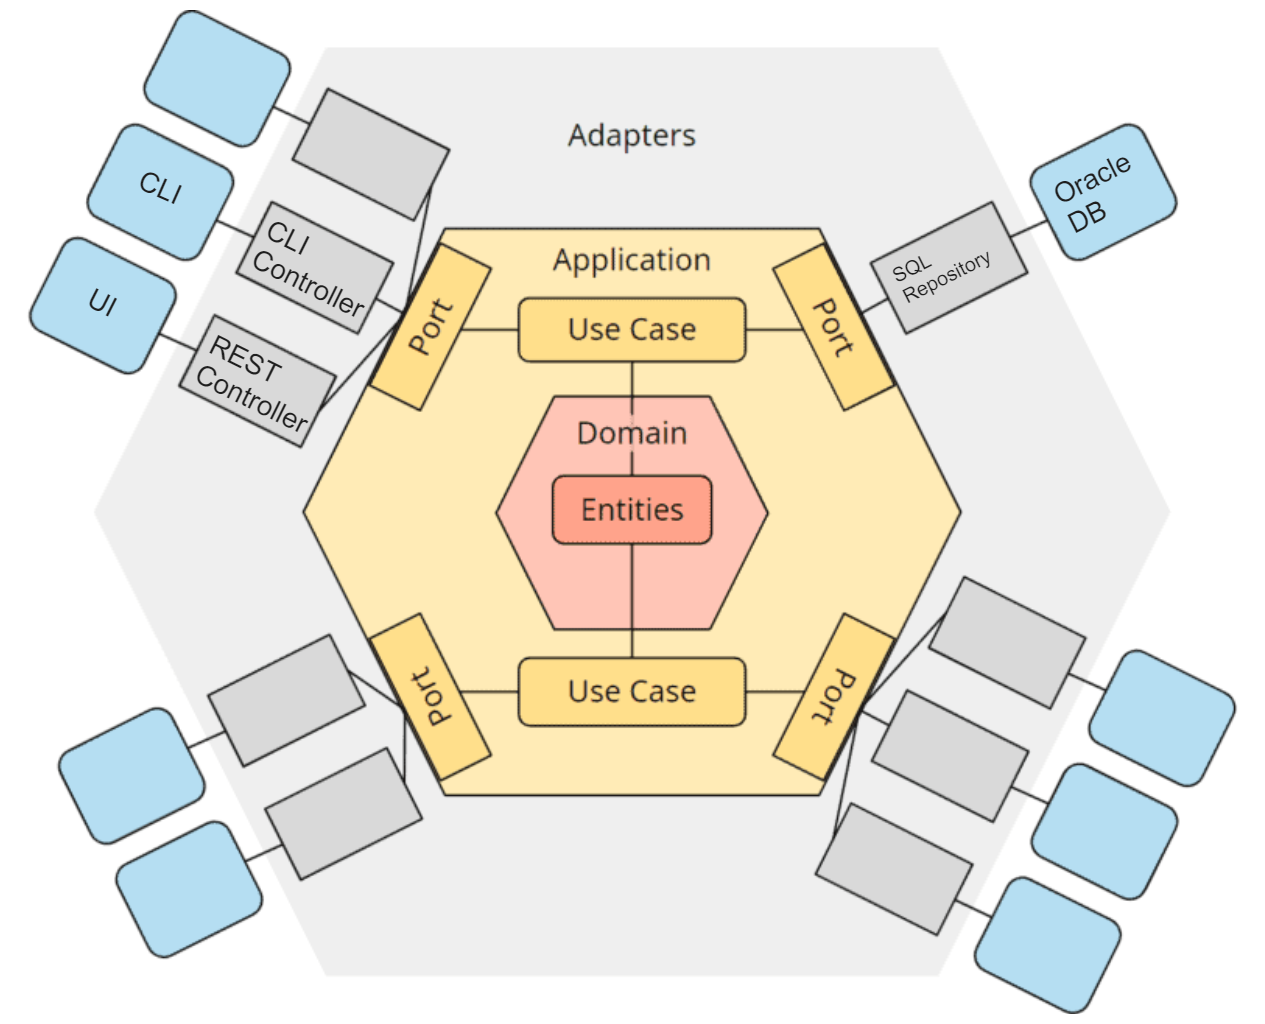
\includegraphics[width=0.8\linewidth]{figuras/hexagonal.png}
    \caption{Hexagonal Architecture visualization from \cite{happycoders2024hexagonal} adapted.}
    \label{fig:hexagonal}
\end{figure}


\section{Frontend architecture}
\paragraph{} Different from FENCE where pages were static and server-side rendered, the team decided to create single page applications (SPAs) that would consume the API endpoints exposed by the backend using FRAPI. A one-page application is a type of web application that interacts with the user by dynamically rewriting the current page rather than loading entire new pages from the server. This approach avoids interruption of the user experience between successive pages, making the application behave more like a desktop application within a web browser \cite{Adobe2023SPAs}.

\paragraph{} In a single-page application, all necessary HTML, JavaScript, and CSS code is either retrieved with a single page load or the appropriate resources are dynamically loaded and added to the page as necessary, usually in response to user actions. The page does not reload at any point in the process, nor does control transfer to another page, although modern web technologies (like HTML5 History API) allow the pages' URL to change without a full page refresh. Single-page applications (SPAs) deliver a fluid user experience by enabling the dynamic updating of webpages. This is achieved through sending requests to the server to fetch data, usually in formats like JSON or XML, and then rendering this data on the client side, which significantly reduces the amount of data transferred between the server and the client, thereby enhancing performance. This client-side rendering approach not only allows for a reduction in the server's workload—since the server is only tasked with sending data in response to requests rather than generating full HTML pages—but also leads to faster server response times and scalability advantages. Reducing the server load is a key advantage for CERN systems due to the geo-distributed user base. SPAs are designed to maintain a continuous user experience by preserving the application's state within the browser, enabling users to experience personalized content and navigate through the application without losing their current state, such as form inputs or scroll position. This stateful interaction, combined with the avoidance of full-page reloads, provides users with a fluid and app-like experience, which is especially advantageous for complex applications that feature rich interactions and workflows.

\paragraph{} Vue.js describes itself in the documentation \cite{VuejsDocumentation} as a progressive JavaScript framework used for building user interfaces chosen for the frontend architecture. It leverages standard web technologies like HTML, CSS, and JavaScript, offering a declarative and component-based programming model that facilitates the development of user interfaces, ranging from simple to complex scenarios. Vue.js is designed to enhance standard HTML with a template syntax that allows developers to declaratively specify HTML output based on JavaScript state, coupled with a reactivity system that automatically updates the DOM in response to state changes.

\paragraph{} The framework's progressive nature means it can be adopted incrementally, fitting various use cases from enhancing static HTML to powering complex Single-Page Applications (SPAs). SPAs benefit significantly from Vue.js due to its efficient update mechanisms and component-based architecture, enabling dynamic content loading and interaction without page reloads. Vue 2 uses the options API for defining component logic. This API uses a descriptive object to define state, methods, and lifecycle hooks. In Glance applications, which require a build step, components are authored using Single-File Components (SFCs). A Single-File Component in Vue.js encapsulates a component's template, logic, and styles within a single file, promoting a cohesive and modular approach to building web applications. Vue.js, coupled with its ecosystem tools such as Vue Router for client-side routing and Vuex for state management, offers a straightforward and well-documented development experience. These characteristics, along with Vue's simplicity, lightweight nature, and growing adoption—especially in comparison to heavier frameworks like React—were pivotal in the decision to utilize Vue.js for the frontend development of the new application as described by Michelly on \cite{michelly}.  

%\paragraph{} The todo list application component presented (based on \cite{vuejs2023sfc}) exemplifies the structure of a Vue.js component built with the Options API. It utilizes the BaseInputText component for the input field, allowing users to type in new todo items. Upon submission, each new item is rendered on the screen using the TodoListItem component, which displays the todo text and provides functionality to remove it from the list. This component could be integrated within a single-page application (SPA) as a route-specific view by leveraging Vue Router, Vue.js's official library for web application routing. Vue Router enables the mapping of different URLs to various components within the SPA, allowing the todo list component to be displayed when a user navigates to a specific URL, for instance, /todos. The router views are rendered in the place of a <router-view> element, and Vue Router handles the intricacies of browser history navigation and URL synchronization. Furthermore, the use of Vue's Slot API within the todo component adds a layer of flexibility, making it highly customizable. For example, by wrapping the BaseInputText with a slot, users of the todo component can replace the default input with their own customized input component or add additional HTML or Vue components around the input area. This could be particularly useful if there's a need to extend the functionality of the input, such as adding date pickers, dropdowns for categories, or tags for the todos. When discussing the Super Search implementation, the flexibility provided by slots will be leveraged to create simple and advanced search interfaces.

\paragraph{}The todo list application component, highlighted in the Vue.js script \ref{lst:vue-script} and template code \ref{lst:vue-template}, demonstrates basic use of Vue.js's Options API, integrating various features that illustrate the component's anatomy. This example is based on a live demo application provided in the Vue official documentation \cite{vuejs2023sfc}.

\paragraph{} Starting with the template structure (Vue.js template code with slot on listing \ref{lst:vue-template}), it defines the HTML markup, binding it to the Vue instance's data or methods (lines 5 to 8 of listing \ref{lst:vue-template}). The greeting message is dynamically rendered based on the computed property \verb|greetingMessage|, showcasing Vue.js's reactive data binding capabilities. The template further introduces a slot around the \verb|BaseInputText| component (Lines 4-10 of listing \ref{lst:vue-template}), enabling custom input content. This use of slots underscores Vue's flexibility and reusability, allowing developers to inject customized content or components into predefined placeholders.

\paragraph{} In the script section of \ref{lst:vue-script}, the code begins importing the \verb|BaseInputText| and \verb|TodoListItem| components (lines 2 and 3 of listing \ref{lst:vue-script}), which are required for inputting new todos and listing them respectively. This exemplifies the component-based architecture of Vue.js, where smaller, reusable components are composed to build more complex components and views. The script delineates props such as \verb|inputPlaceholder| and \verb|emptyListMessage|, which are custom attributes designed for facilitating data transfer from parent to child components. In the component illustrated in listing \ref{lst:vue-script}, the \verb|inputPlaceholder| prop is bound to the \verb|BaseInputText| component's \verb|placeholder| prop. Consequently, modifying the value of \verb|inputPlaceholder| automatically propagates the changes to the \verb|placeholder|.

\paragraph{} The data function (line 14 of listing \ref{lst:vue-script}) declares the local state of the component, including \verb|newTodoText| and \verb|todos|, illustrating the reactive state management in Vue.js. Through methods (lines 20 to 28 of listing \ref{lst:vue-script}) like \verb|addTodo| and \verb|removeTodo|, the state is manipulated, reflecting changes in the UI without direct DOM manipulation, showcasing Vue's declarative rendering capabilities.

\paragraph{}  Computed properties (line 29 of listing \ref{lst:vue-script}), such as \verb|greetingMessage|, dynamically calculate values based on reactive data, offering a cached, efficient way to update the UI based on state changes. Watchers (script \ref{lst:vue-script} line 34) on properties like \verb|todos| provide a mechanism to perform actions in response to state changes.

\paragraph{} Lifecycle hooks (script \ref{lst:vue-script} lines 39 to 44), including \verb|created| and \verb|mounted|, offer insights into the component's lifecycle stages, allowing for initialization tasks and DOM manipulations post-rendering. This demonstrates the control Vue provides over a component's lifecycle, allowing developers to hook into key events.

\paragraph{} Vue also provides tools to define scoped styles, which are applied only to the component defined in the same file as the style. This is shown in the code \ref{lst:vue-style}.

\paragraph{} Finally, an integration with Vue Router would enable this component to be part of a SPA, mapping URLs to views/components and rendering them within a \verb|<router-view>| element, facilitating SPA development with Vue.js. Vue Router's handling of browser history and URL synchronization enhances the SPA navigability and allows users to use the browser's back button. Image \ref{fig:todo-app} illustrates what the component created looks like.


\begin{lstlisting}[language=HTML, caption=Vue.js template code with slot., label=lst:vue-template]
<template>
  <div>
    <h1>{{ greetingMessage }}</h1>
    <slot name="input">
      <BaseInputText 
        v-model="newTodoText"
        :placeholder="inputPlaceholder"
        @keydown.enter="addTodo"
      />
    </slot>
    <ul v-if="todos.length">
      <TodoListItem
        v-for="todo in todos"
        :key="todo.id"
        :todo="todo"
        @remove="removeTodo"
      />
    </ul>
    <p v-else>
      {{ emptyListMessage }}
    </p>
  </div>
</template>
\end{lstlisting}


\begin{lstlisting}[language=javascript, caption=Vue.js script code., label=lst:vue-script]
<script>
import BaseInputText from './BaseInputText.vue'
import TodoListItem from './TodoListItem.vue'

export default {
  components: {
    BaseInputText,
    TodoListItem
  },
  props: {
    inputPlaceholder: String,
    emptyListMessage: String
  },
  data() {
    return {
      newTodoText: '',
      todos: []
    }
  },
  methods: {
    addTodo() {
      this.todos.push({ id: this.nextTodoId++, text: this.newTodoText });
      this.newTodoText = '';
    },
    removeTodo(idToRemove) {
      this.todos = this.todos.filter(todo => todo.id !== idToRemove);
    }
  },
  computed: {
    greetingMessage() {
      return `You have ${this.todos.length} todos`;
    }
  },
  watch: {
    todos(newTodos) {
      console.log('The todo list has changed!', newTodos);
    }
  },
  created() {
    console.log('Component has been created');
  },
  mounted() {
    console.log('Component has been mounted to the DOM');
  }
}
</script>
\end{lstlisting}

\begin{lstlisting}[language=HTML, caption=Vue.js style code., label=lst:vue-style]
<style scoped>
button {
  font-weight: bold;
}
</style>
\end{lstlisting}
\begin{figure}[H]
    \centering
    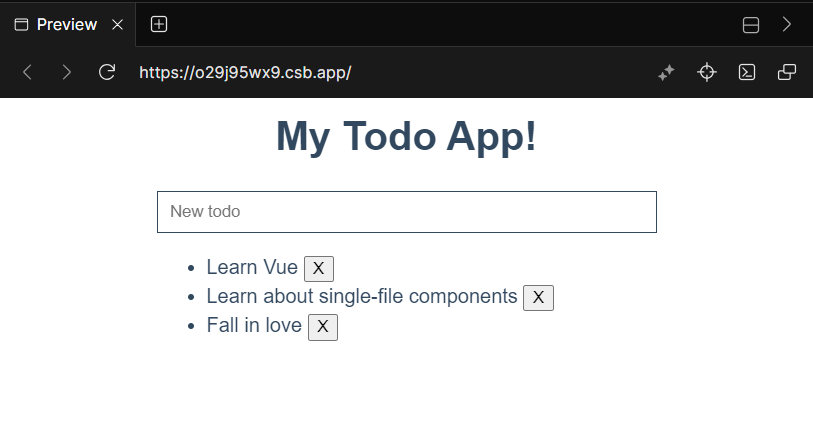
\includegraphics[width=0.8\linewidth]{figuras/todo-app.png}
    \caption{Todo Vue app example.}
    \label{fig:todo-app}
\end{figure}


%\subsection{vuex}

\paragraph{} In the project's early stages, the developers embarked on creating a suite of components that would serve as the foundational building blocks for new systems. This suite encompassed a variety of elements, such as text inputs, tables, and navigation bars, among others. Complementing these components, the team crafted a dedicated plugin to handle user authentication, all of which were consolidated into a JavaScript library named fence-vue. Despite this effort, the developers recognized the existence of numerous established libraries offering similar functionalities, moved by vast and active communities. A notable example is Vuetify—a material design UI framework built atop Vue.js. Vuetify stands out by providing an extensive array of pre-designed, customizable components and directives that expedite the process of creating aesthetically pleasing and responsive web applications. One of the significant benefits of Vuetify is its integration with Figma, a web-based collaborative tool for UI/UX and graphic design that facilitates real-time teamwork. With its Figma components, Vuetify enables developers to swiftly prototype and iterate on interface designs, ensuring a smooth design-to-development workflow and fostering a more agile and collaborative environment. Figure \ref{fig:vuetify} shows some of Vuetify's components on a Figma project. The developers then limited the scope of fence-vue to common plugins and more complex components built on top of Vuetify's base ones.


\begin{figure}[H]
    \centering
    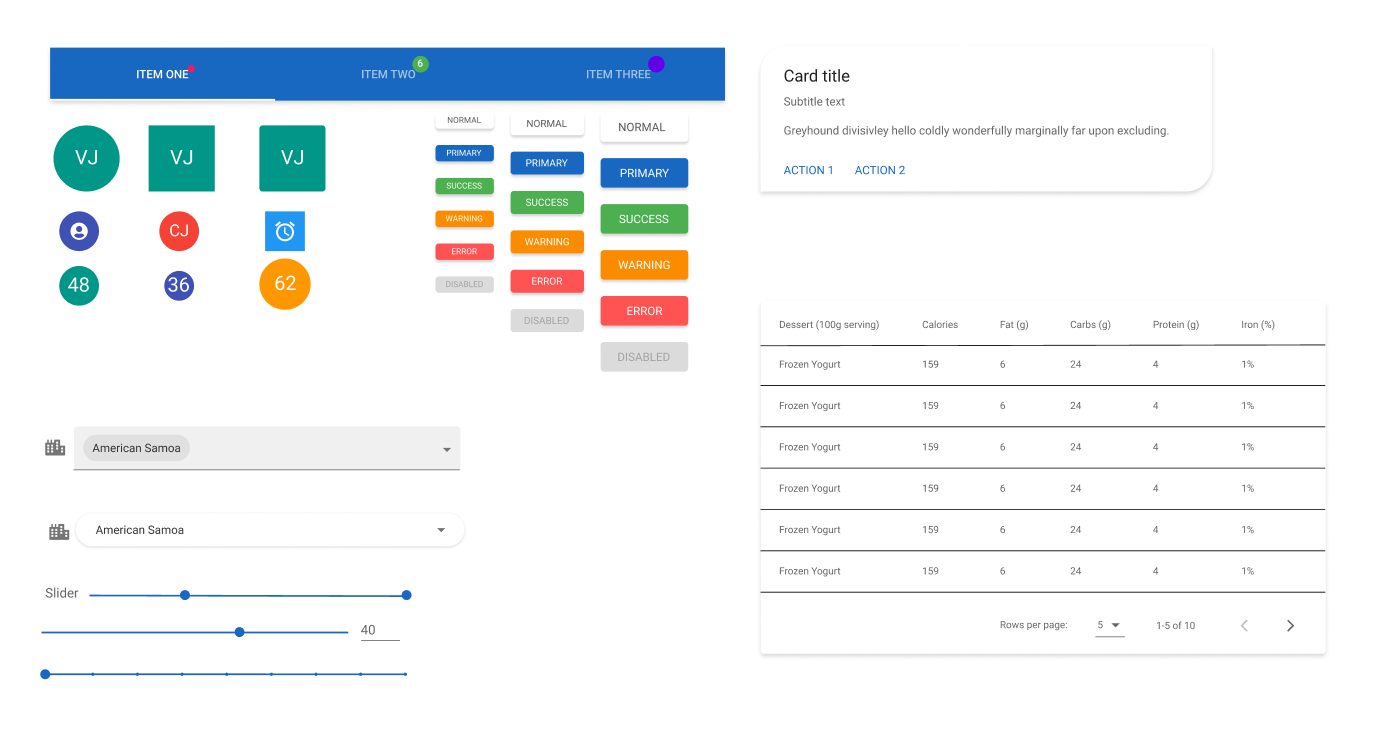
\includegraphics[width=1\linewidth]{figuras/vuetify.png}
    \caption{Some of Vuetify's components shown in Figma.}
    \label{fig:vuetify}
\end{figure}

\section{Authorship Implementation} 

\paragraph{} The Authorship implementation started at the beginning of 2020, following a consensus among stakeholders and developers that the gathered requirements were sufficiently mature. However, the development began during a period when the team was adhering to the Layered Architecture model. This timing resulted in certain inconsistencies within the system's design. Notably, newer features implemented after the initial deployment to production had already transitioned to following the Hexagonal Architecture, leading to a mix of architectural approaches.

\paragraph{} Upon starting a new project, it's necessary to register the new application on the CERN applications portal. This involves registering two separate applications: one for the frontend and another for the API, which is important for creating the needed credentials to safely communicate between the two. After registering the application, the next step is to add a new CERN SSO Registration. When doing this, developers need to keep in mind that: for client applications, they must choose the option ``my application cannot store a client secret safely" to make it a public client, which means only a Client ID will be needed. For APIs, especially if the application needs to talk to secure CERN APIs like the Authz Service API, they might need to select the option that allows generating tokens, useful for tasks such as adding or removing members from a GRoups for APPlications Authorization (GRAPPA) Group. This registration process provides the required credentials (Client ID and Client Secret) for applications to authenticate users through the OAuth 2 protocol.

\paragraph{} E-Groups serve as the foundational system at CERN for granting user access to applications through membership in various groups, integrated within the Single Sign-On (SSO) tokens. Utilized extensively within the organization, E-Groups facilitate authorization in a recursive manner, allowing a single e-group to be associated with multiple other e-groups. The GRAPPA system is introduced as a modern replacement for E-Groups, aiming to address and improve upon the limitations of the previous authorization infrastructure. In the Authorship context, for example, there is a GRAPPA Group for the LHCb Glance Developers. This group is then used to grant the \verb|admin| \textbf{role} to the developers in the application's settings. Roles can be defined on a user basis or based on Grappa groups. Another example of group is the LHCb Secretariat which grants the \verb|secretariat| role in the Membership and Authorship systems.

\paragraph{} The general application folder structure has three main directories:
\dirtree{%
.1 api.
.1 client.
.1 database.
}

The \verb|api| directory houses the entire backend codebase, predominantly comprised of PHP classes. This structure facilitates the separation of concerns by ensuring that all server-side logic and data manipulation tasks are centrally managed. Conversely, the \verb|client| directory is dedicated to the frontend development aspects, encompassing Components, views, and styles to create user interfaces. Additionally, the \verb|database| directory contains SQL migration files, which play an important role in managing database schema changes and ensuring data consistency across different stages of the application's lifecycle.

\subsection{The Authorship Backend}

\paragraph{} FRAPI-based applications tend to have a similar backend structure. Expanding the \verb|api| folder content, the following subfolders can be found:

\dirtree{%
.1 api.
.2 configuration.
.2 routes.
.2 docs.
.2 resources.
.3 notifications.
.3 templates.
.3 queries.
.4 delete.
.4 insert.
.4 select.
.4 update.
.3 schemas.
.2 src.
.3 AuthorsList.
.4 Application.
.5 DeleteAcknowledgement.
.5 DeleteFundingAgency.
.5 GetAcknowledgementTex.
.5 GetAuthorsList.
.5 GetFundingAgencyDetails.
.5 GetGrantDetails.
.5 GetInternationalOrganizationDetails.
.5 RegisterAcknowledgement.
.5 RegisterAuthorsListForPaper.
.5 RegisterFundingAgency.
.5 RegisterGrant.
.5 Subscribers.
.5 UpdateGrant.
.4 Domain.
.5 Event.
.4 Infrastructure.
.4 Cronjob.
.4 Persistence.
.4 Web.
.3 Controllers.
.3 Cronjob.
.3 DTO.
.3 Models.
.3 Persistence.
.3 Notifications.
.3 Repositories.
.3 Services.
.3 tests.
.4 Comparison.
.4 Integration.
}

\paragraph{} Inside the \verb|configuration| folder, it is required to add an \verb|api.json| configuration file. This file includes authentication settings, such as defining which SSO provider will be used by FRAPI and the API public endpoints' paths.

\paragraph{} SSO is an authentication process that allows a user to access multiple applications or systems with one set of credentials, thus eliminating the need to log in separately to each system. SSO can be implemented using various authentication protocols, including SAML (Security Assertion Markup Language), OAuth, and OpenID Connect. At CERN, OAuth 2 was the protocol used provided by Keycloak: an open-source Identity and Access Management solution developed by Red Hat.


\paragraph{} In the \verb|api.json| it is also included the path for the User class, which defines a set of properties required for every authenticated user to record the actions performed by them and perform authorization checks. For the Authorship and the Membership the User class has the following properties: \verb|$id|, \verb|$appointments|, \verb|$primaryEmployment|, and \verb|$cernId|.

\paragraph{} In this file it is also provided the Sentry instance URL in case the application has one. Sentry is an open-source error-tracking software that provides monitoring and fixing of crashes in real time. It enables the detection, understanding, and resolution of issues affecting the user experience through detailed error insights. Sentry facilitates the identification of the specific line of code causing an issue, the conditions under which the error occurred, and its impact on users. This capability assists developers in addressing problems promptly, potentially before users notice them.

\paragraph{} Within the \verb|configuration\routes| directory, each API endpoint is mapped to its corresponding controller method handler. This directory contains a JSON file for each resource, which is read by FRAPI. It subsequently manages the routing of requests to the appropriate controller methods based on this configuration. As shown in the JSON \ref{lst:AuthorsListRoute} line 13, it is possible to provide an array of roles required to access a given resource. If the user tries to access a resource without the correct permission, FRAPI will return a response with HTTP status code 401: unauthorized.

\paragraph{} FRAPI also implements a middleware for JSON schema validation which ensures JSON documents (in the REST API context, the request body) adhere to a predefined structure, defined by a JSON Schema. This includes constraints on data types, properties, and formats. The schema, written in JSON, specifies properties, required fields, value constraints, and array items, among other rules. Validation occurs at runtime, safeguarding against errors and vulnerabilities by verifying data conformity. When the payload received does not pass the schema validation, FRAPI will automatically respond with a 400 Bad Request error indicating a problem with the client's request to the server specifying which fields did not pass the schema validation.

\paragraph{} The \verb|authorization| field (code \ref{lst:AuthorsListRoute} line 8) is used to provide the list of required groups a user must belong to in order to access the given endpoint.

\paragraph{}

\begin{lstlisting}[language=javascript, caption=authors list resource routes., label=lst:AuthorsListRoute]
{
    "type": "controller",
    "class": "\\LHCb\\Membership\\Controllers\\AuthorsListController",
    "paths": {
        "/authors-lists": {
            "GET": {
                "method": "getAllAuthorslistBasicInformation",
                "authorization": ["basic-user"]
            },
            "PATCH": {
                "method": "update",
                "authorization": ["editorial-board-member"],
                "schema": "resources/schemas/authorslist-update.json"
            }
        },
        "/authors-lists/institutes": {
            "GET": {
                "method": "getAllInstitutes",
                "authorization": ["basic-user"]
            }
        }
        ...
\end{lstlisting}

\paragraph{} Inside the \verb|api/docs| folder it is stored the Swagger Documentation to facilitate external systems to connect to the APIs. Swagger, as described on \cite{SwaggerDocs}, is a toolset that supports the OpenAPI Specification (OAS) for developing APIs. It enables the description of the structure of APIs, making it possible for both humans and computers to understand the capabilities of a service without accessing its source code. Swagger facilitates the documentation, client SDK generation, and API testing by providing a specification that can be used to describe APIs. This specification is written in either YAML or JSON format and includes details such as available endpoints, operations, parameters, and responses. Swagger also supports API authentication mechanisms and the description of input and output models for API operations. The Membership API Swagger Docs is shown in Figure \ref{fig:swagger}

\begin{figure}[H]
    \centering
    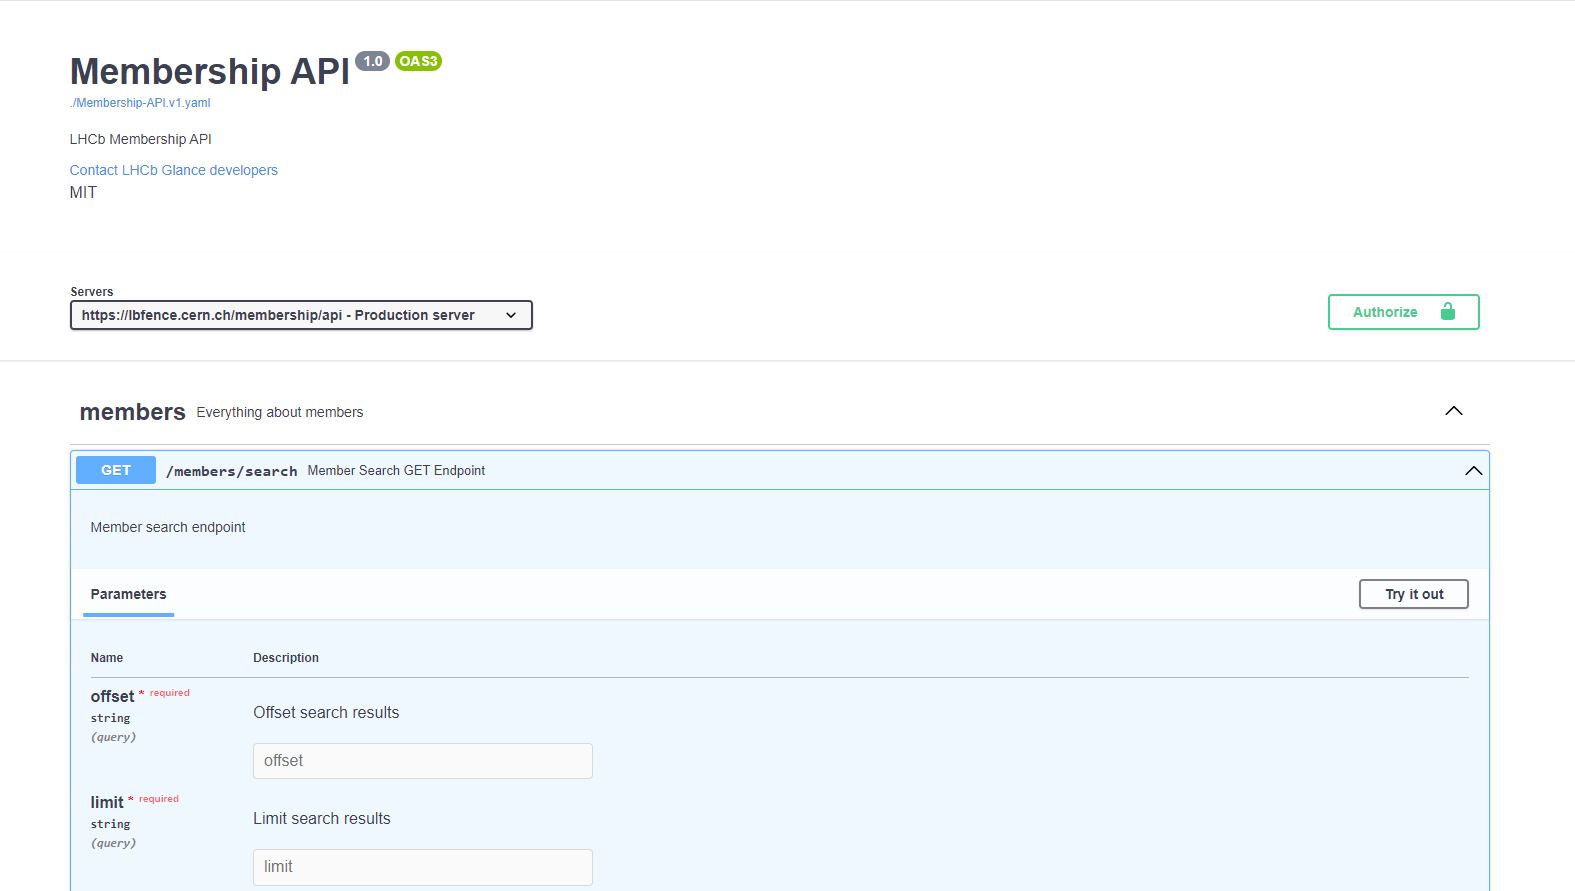
\includegraphics[width=0.8\linewidth]{figuras/swagger.png}
    \caption{API documentation example.}
    \label{fig:swagger}
\end{figure}


\paragraph{} The \verb|api/resources| directory is a repository for various non-PHP class API components. The \verb|api/resources/notifications| directory encompasses JSON configuration files that detail the subject and the corresponding HTML template for notifications. Furthermore, \verb|api/resources/templates| houses both HTML and LaTeX templates—the latter being utilized by PHP classes for generating Authorship .tex files. Additionally, the resources directory contains SQL queries employed by Repositories for database operations such as reading, writing, updating, and deleting data, as well as JSON schemas for validating request structures.

\paragraph{} The \verb|src| directory is where all PHP code within the project lives. As previously explored, the backend implementation adopts two distinct architectural patterns: the layered architecture on the left, and the hexagonal architecture on the right. The fundamental distinction between these two approaches lies in the location and application of business logic within the system's structure. Both approaches share similarities such as the Controller classes which process the request routed to them by FRAPI. They also use the Repository Pattern: a design pattern used to manage data access logic in a centralized location. It acts as an abstraction layer between the domain model (the core business logic of your application) and the persistence layer (the mechanism used to store and retrieve data, like databases or files).

\paragraph{}

\begin{minipage}{.5\textwidth}
\dirtree{% First directory structure
.2 src.
.3 Persistence.
.3 Controllers.
.3 Cronjob.
.3 DTO.
.3 Models.
.3 Repositories.
.3 Services.
}
\end{minipage}%
\begin{minipage}{.5\textwidth}

\dirtree{% Second directory structure (Duplicate of the first for demonstration)
.2 src.
.3 AuthorsList.
.4 Application.
.5 DeleteAcknowledgement.
.5 DeleteFundingAgency.
.5 GetAcknowledgementTex.
.5 GetAuthorsList.
.5 ....
.5 Subscribers.
.4 Domain.
.5 Event.
.4 Infrastructure.
.4 Cronjob.
.4 Persistence.
.4 Web.
.3 Notifications.
.3 Shared.
.4 ....
}
\end{minipage}

\paragraph{} In the Layered Architecture, the \verb|src\Controllers| directory is designated for storing Controller classes. These controllers are responsible for initiating a Data Transfer Object (DTO) when required (specifically for write or update operations) and subsequently invoking a Service class. The Service class implements the core business logic pertinent to a particular domain. The \texttt{src/Services/AuthorsList\-Service.php}, for instance, exposes a series of methods to Controllers, including but not limited to:
\begin{enumerate}
    \item \verb |getAuthorsList|: This method constructs an instance of the \path{src/Models/AuthorsList.php} class, populates it with data regarding authors and institutes, processes all the information (sorts authors, assign indexes), and delivers the assembled list back to the Controller. The Controller then serializes this list for inclusion in the response to a request.
    \item \verb|downloadAuthorsList|: Similar in functionality to \verb|getAuthorsList|, this function also compiles the authors list but differs in its output by generating a downloadable file in a specified format (e.g., PDF or .tex).
    \item \verb|insert|: This method accepts an \verb|AuthorsListInputDTO|, performs validation on it, and, if the data is deemed valid, it proceeds to persist this information through a call to the Repository dependency.
    \item \verb|getNonAuthors|: It invokes the Repository dependency to retrieve a list of members who do not qualify as authors. This functionality is particularly useful for identifying all Members eligible to be considered as exceptions.
\end{enumerate}

\paragraph{} The main issue with this approach is that the Service classes quickly grew large and became hard to maintain. This was partly caused by the fact that the classes inside the Model namespace (\verb|src/Models|) were anemic models which are considered an anti-pattern associated with object-oriented programming, particularly in the context of Domain-Driven Design (DDD) lacking significant or relevant behavior, primarily focusing on holding data with minimal or no business logic encapsulated within it.

\paragraph{} In the Hexagonal Architecture, on the other hand, there are multiple \textbf{Handler}s that process \textbf{Command}s for write operations. Controllers also have direct access to Repository interfaces so that simple operations (such as the \verb|getNonAuthors| use case) don't require a Handler for them. This approach also moves the core business logic to the Domain. In this approach, the \verb|getAuthorsList| use case starts with a request routed to a Controller method, which uses one of its N Handler dependencies, the Handler gathers all the information from the Persistence source with its Repository dependencies and supplies the \verb|\src\AuthorsList\Domain\AuthorsList| class with this information \textbf{for it to process}. Similarly, in the \verb|insert| use case, the Handler will only perform persistence-dependent validations (checking if the provided ID is unique, for example) and most of the business validation is performed in the \verb|\src\AuthorsList\Domain\AuthorsList| constructor.

\paragraph{} The following code excerpts illustrate the difference between the mentioned architectures by giving a general overview of the \verb|downloadAuthorsList| use case, which was first developed using the Layered Architecture and then migrated to the Hexagonal.

\begin{lstlisting}[language=PHP, caption={Layered Architecture Implementation.}, label=lst:layer]
// \src\Controllers\AuthorsListController.php
public function getAuthorsListForGivenPaper(Api $api, $id) {
    $authorsList = $this->authorsListService->getAuthorsList($id);
    $json = json_encode($authorsList->serialized());
    $response = $api->getResponse();
    $response->getBody()->write($json);
    return $response->withHeader("Content-Type", "application/json");
}

// \src\Services\AuthorsListService.php
public function download($id, $extension, $agentId, $date = null) {
    if ($id) {
        $authorsList = $this->getAuthorsList($id);
    } else {
        $authorsList = $this->getAuthorsListForGivenDate($date);
    }
    $data = $authorsList->serialized();
    return AuthorsListFilesHandlerService::download($extension, $data, $agentId);
}

public function getAuthorsList($id) {
    $authorsList = $this->_repository->build($id);
    if ($authorsList->hasPublishedInformation()) {
        return $authorsList;
    }
    return $this->getAuthorsListWithAssignedIndexes($authorsList);
}

private function getAuthorsListWithAssignedIndexes(AuthorsList $authorsList): AuthorsList {
    $authors = $this->getAuthors($authorsList->getReferenceDate(), $authorsList->getId());
    $institutes = $this->getInstitutes($authors, $authorsList->getReferenceDate());
    $institutes = $this->setInstitutesIndexes($institutes, $authorsList->getReferenceDate());
    $authors = $this->setAuthorsIndexes(
        $institutes["institutes-dictionary"], 
        $authors, 
        $authorsList->getReferenceDate()
    );
    $authorsList->setAuthors($authors);
    $exceptions = $authorsList->getExceptionsAuthor();
    if ($exceptions) {
        $exceptions = $this->setExceptionsIndexes(
            $institutes["institutes-dictionary"], 
            $exceptions, 
            $authorsList
        );
        $authorsList->setExceptionsAuthor($exceptions);
    }
    $authorsList->setInstitutes($institutes["sorted-institutes"]);
    return $authorsList;
}
\end{lstlisting}

In a Layered Architecture model, the interaction between the Controller and the Service layer is very close, as the latter encapsulates the majority of the application's business logic. This design paradigm often results in the consolidation of business logic within the Service layer, giving rise to voluminous, monolithic service classes. This complexity is illustrated in code \ref{lst:layer} (lines 11 to 49), where the Service initially determines whether to construct an AuthorsList for a paper or for a specific date (defaulting to the authors for the date). It then retrieves all requisite data from Repositories and processes it. This processing entails assigning indices to Institutes based on predefined rules, associating these indices with the Authors, organizing Authors and Institutes, and finally, transferring this processed data to the \verb|src/Models/AuthorsList.php| class. Rather than functioning as a domain model, this class primarily acts as a data serializer, further highlighting its anemic behavior.

\begin{lstlisting}[language=PHP, caption={Hexagonal Architecture Implementation.}, label=lst:hexagonal]
// \src\AuthorsList\Infrastructure\Web\AuthorsListController.php
public function downloadAuthorsList(Api $api, string $extension, int $id) {
    $agentId = (int) $api->getUser()->getPersonId();
    $authorsList = $this->downloadAuthorsListHandler->handle($id, $extension, $agentId);

    $response = $api->getResponse();
    $response = $response->withHeader("Content-Type", Mime::fromExtension($extension));
    $response = $response->withAddedHeader("Content-Disposition", "attachment");
    $response->getBody()->write($authorsList);

    return $response;
}

// \src\AuthorsList\Application\DownloadAuthorsList\DownloadAuthorsListHandler.php
public function handle(int $authorsListId, string $extension, int $agentId) {
    $authorsList = $this->repository->findAuthorsListById($authorsListId);
    $authorsList->computeAuthorsList();
    return AuthorsListFilesHandlerService::download($extension, $authorsList->serialized(), $agentId);
}

//  \src\AuthorsList\Domain\AuthorsList.php
public function computeAuthorsList(): void {
    $this->computeInstitutesIndexes();
    $this->computeAuthorsIndexes();
    $this->computeExternalAuthorsIndexes();
    $this->sortAllAuthors();
}
\end{lstlisting}

\paragraph{} In the code snippet (\ref{lst:hexagonal}), the distribution of tasks is optimized, facilitating a clearer comprehension of the procedure for assembling the authorship list. Similar to the Layered Architecture approach, the request navigates to the Controller via FRAPI, which now interfaces with various Handlers, such as but not limited to:
\begin{itemize}
    \item \verb|RegisterAuthorsListForPaperHandler|
    \item \verb|UpdateGrantHandler|
    \item \verb|DownloadAuthorsListForGivenDate|
    \item \verb|GetNonAuthors|
    \item \verb|RegisterAcknowledgementHandler|
\end{itemize}
\noindent
Upon receiving a request, the Controller engages the appropriate Handler to coordinate the necessary operations to address the request. As delineated in (\ref{lst:hexagonal}), the Handler employs a Repository to create an instance of the \texttt{AuthorsList} class, supplying it with all pertinent data required for the compilation of the list. This includes all Members eligible for authorship, any Exceptions (Authors added or removed), and a catalog of Institutes. Subsequently, the \texttt{AuthorsList} domain class undertakes the processing of this data, thereby consolidating all expertise related to the list's formation within the Domain. The construction of the list is executed via the \texttt{computeAuthorsList} method, which administers a series of sub-tasks to generate and structure the author roster, their affiliations, and external contributors in accordance with a set of criteria and regulations. The methodology is deconstructed into four phases, as illustrated in line 21 of code (\ref{lst:hexagonal}).

\paragraph{} The first step, performed in the \verb|computeInstitutesIndexes|, method involves assigning indexes to each Institute within the list. These indexes are necessary for organizing Institues in a structured way and for referencing them efficiently in other parts of the authors list computation. The algorithm attributes a numeric index to Official and Affiliated institutes and an alphabetical one to the others. Index attribution follows a hierarchical sorting criterion, prioritizing Country, City, and then Institute Name. This systematic ordering culminates in a structured mapping, where each institute is linked to a unique composite ID—integrating both its Id and classification (External or Regular)—and a corresponding index. This associative dictionary facilitates efficient retrieval and linkage between Institutes and their respective Authors.

\paragraph{} After institutes have been indexed, each Author's index is computed based on their Employments with these Institutes. This is first done for regular LHCb Authors (in \verb|computeAuthorsIndexes|) and later for External Authors (in the \texttt{compute\-External\-Authors\-Indexes} method). Authors may be affiliated with one or more Institutes, and their index reflects this association. The index assignment process involves iterating through each Author, determining their affiliated Institute based on the reference date, and then assigning the Institute's index to them, which is done in constant time by accessing the dictionary previously built. This step is important for organizing authors in a way that reflects their professional or academic affiliations accurately. The same process is performed for External Authors.

\paragraph{} Finally, the \verb|sortAllAuthors| function involves sorting all Authors (both internal and external) according to a predefined set of criteria, which includes the index, the alphabetical order of last names, and the initials in this order of priority. 

\paragraph{} Once the list is compiled, the Handler uses a static class (line 18 of code \ref{lst:hexagonal}) to download the serialized content into a given format (PDF, .tex, for example) and passes the content to the Controller which encapsulates it in the response object exposed to the final user through FRAPI again.

\paragraph{} Domain Classes have the capability to emit events, for instance, when a new Grant is registered, the \verb|src\AuthorsList\Domain\Event\NewGrant.php| event is emitted. These events are monitored by Subscribers, as exemplified by those located in \verb|src\AuthorsList\Application\Subscribers|. Subscribers respond to the events they receive, often by initiating notifications through the \verb|src\Notifications| classes. Employing this pattern, commonly seen in multithreaded languages such as C\#, is also beneficial in PHP to enhance the separation of concerns, delegating specific responsibilities to more specialized namespaces.

\paragraph{} The final Authorship Backend aspect are the Cronjob classes inside \texttt{src\textbackslash Cron\-job}. A cron job is a scheduled task in Unix-based systems used for running scripts or commands at specified times and intervals. It leverages the cron daemon, a background process that runs continuously, checking for scheduled tasks to execute. Cron jobs are commonly used for automating system maintenance, monitoring tasks, and routine backups. The scheduling of a cron job is defined in a cron table (crontab), which specifies the execution time and command to be run. In the Authorship context, cronjobs are used to send notifications when a Grant is about to expire. 


\paragraph{} The authorship generation process is designed to be deterministic, ensuring that identical commands (e.g., \verb|$authorsListId|) consistently produce the same author list. Due to a stringent deadline for project delivery, unit testing was not conducted. Instead, an integration test suite was developed within the \verb|src/Integration| namespace. This suite performs end-to-end testing to verify the responsiveness of all endpoints to simulated requests. Additionally, the \verb|src/tests/Comparison| namespace contains a series of end-to-end tests designed to ensure the stability of the Authors List's content amidst code changes. These tests generate the authorship list in various formats and compare the output against a predefined, accurate version. 

\paragraph{} In contrast to the FENCE applications, which lacked a clear separation of concerns, leading to the necessity of deploying applications on a testing server for manual validation of changes, the current approach allows for backend modifications to be automatically verified. This is achieved by executing the Integration test suite through the GitLab CI/CD (Continuous Integration/Continuous Deployment) tools. GitLab CI/CD provides a framework for automating the testing and deployment processes. It facilitates the execution of predefined test suites upon each commit, ensuring that any code alterations do not break the existing functionality. Figure \ref{fig:pipeline} shows a merge request that passed the integration tests. 

\begin{figure}[H]
    \centering
    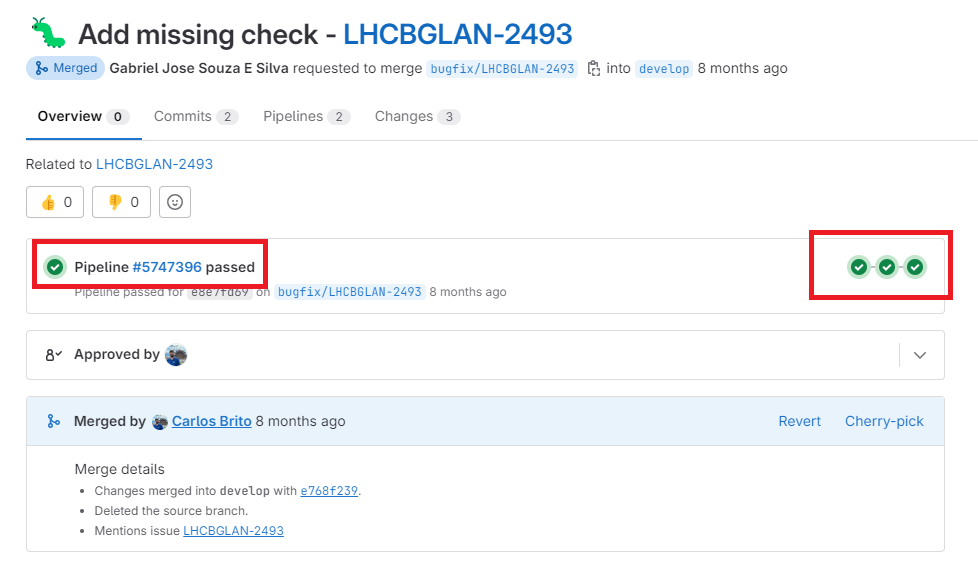
\includegraphics[width=0.8\linewidth]{figuras/tcc_pipeline.png}
    \caption{Gitlab Pipeline passing on Merge Request. The pipeline steps include building the backend API with \texttt{composer install}, building the frontend with \texttt{npm run build}, and running the backend integration test suite.}
    \label{fig:pipeline}
\end{figure}





\subsection{The Authorship frontend}

\paragraph{} The frontend of the Authorship System is housed within the \verb|client| directory. 

\dirtree{%
.1 client.
.2 public.
.2 src.
.3 api.
.3 assets.
.4 css.
.4 images.
.3 components.
.3 mixins.
.3 plugins.
.3 router.
.3 store.
.4 modules.
.3 views.
.4 authorsList.
}

\paragraph{} Within this directory, the \verb|client/public| folder contains the application's entry point HTML file, which is automatically generated by utilizing the Vue Command Line Interface (CLI) via the \verb|vue create| command. The \verb|assets| folder, also located within the \verb|client| directory, stores static assets utilized by the frontend. These assets include CSS style sheets that are applied globally across all components and static images, such as the LHCb collaboration logo and the homepage banner.

\paragraph{} The \verb|components| folder houses the fundamental building blocks of the user interface, akin to the example provided in the todo application illustrated in code \ref{lst:vue-script}. The guiding philosophy for developing components was to resort to custom creation only when the pre-existing components from Vuetify failed to meet specific needs or when it was necessary to combine several Vuetify components to build a more complex one. For instance, Image \ref{fig:tcc_latex_title} showcases a custom component designed to accept a LaTeX expression through its props and render the corresponding text. Conversely, Figure \ref{fig:tcc_loading} depicts a custom component crafted by integrating Vuetify's \verb|VDialog|, which generates the modal window, with Vuetify's \verb|VProgressLinear| to visually signify the loading process. The second one is displayed whenever a user triggers an action and the interface must wait for the response.


\begin{figure}[H]
    \centering
    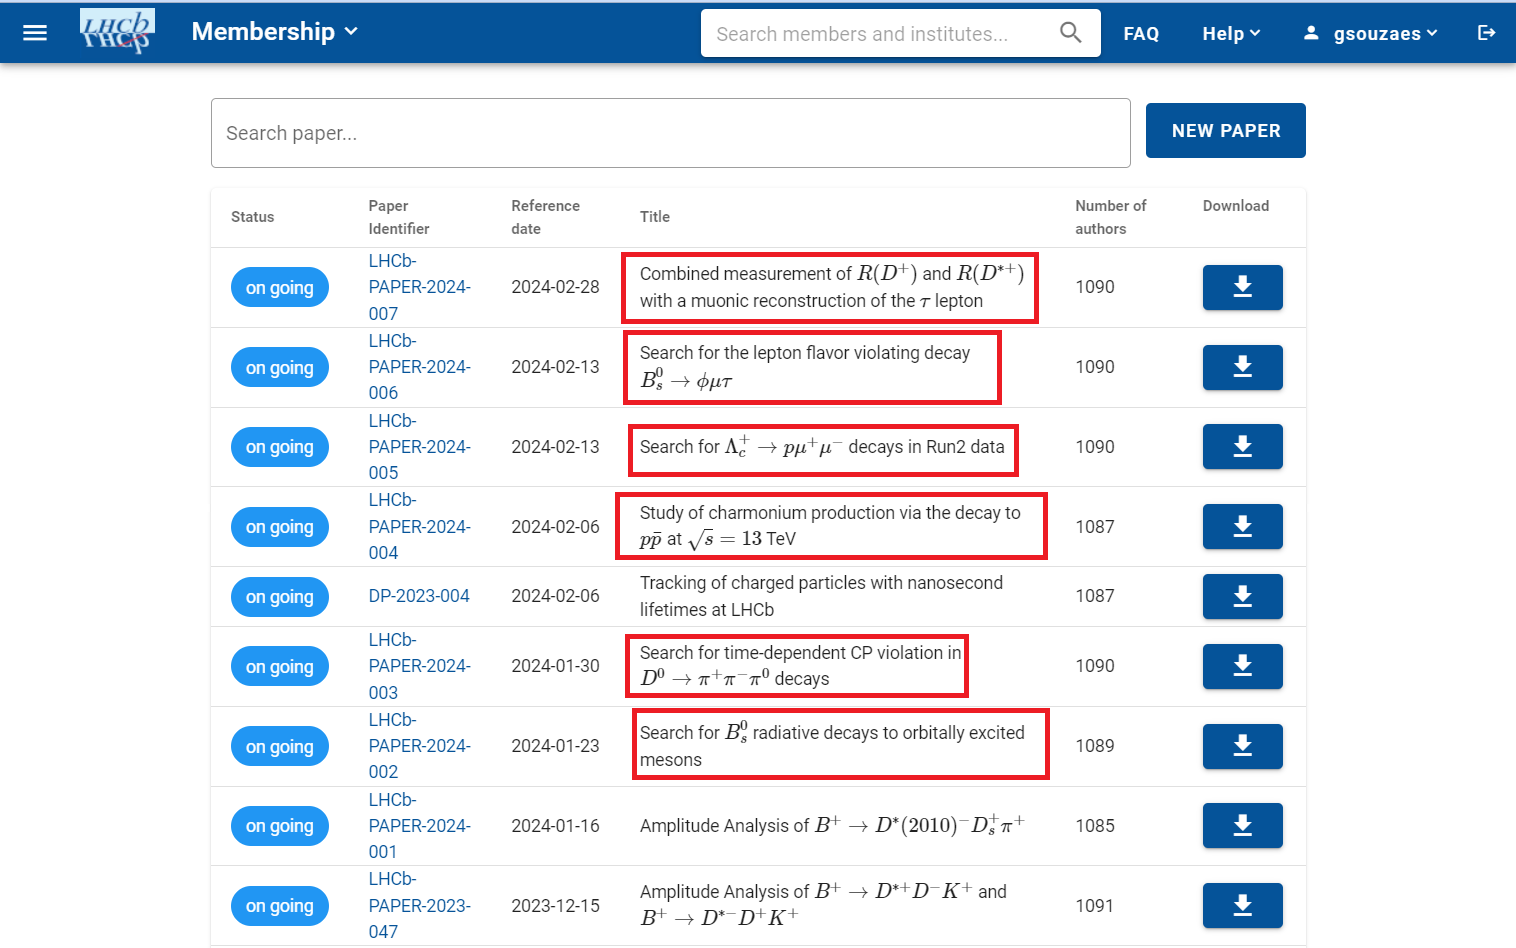
\includegraphics[width=0.9\linewidth]{figuras/tcc_authorship_home.png}
    \caption{\texttt{LatexTitle.vue}: Textual component to process latex code.}
    \label{fig:tcc_latex_title}
\end{figure}


\begin{figure}[H]
    \centering
    
\includegraphics[width=0.5\linewidth]{figuras/tcc_loading.png}
    \caption{\texttt{LoadingModal.vue}: Loading popup component.}
    \label{fig:tcc_loading}
\end{figure}

\paragraph{} Vue Mixins are stored in the \verb|client/mixins| path. A mixin object can contain any component options. When a component uses a mixin, all options in the mixin will be ``mixed" into the component's own options. This approach allows for a form of ``soft" inheritance, enabling component reuse without requiring complex inheritance structures. These scripts can include a wide range of component options such as data, methods, lifecycle hooks (e.g., created, mounted), computed properties, and watchers. When a component uses a mixin that contains a lifecycle hook, the mixin's hook is called before the component's own hook if both are defined. A very used mixin in Glance applications is shown in code \ref{lst:mailto} which injects a method in all components that import it that generates a clickable email link based on a list of emails.

\begin{lstlisting}[language=javascript, caption={Mailto Mixin.}, label=lst:mailto]
export default {
    methods: {
        getMailto(emails) {
            const localMails = !Array.isArray(emails) ? [emails] : emails;
            return `mailto:${localMails.join(',')}`;
        },
    },
};
\end{lstlisting}

\paragraph{} Inside the \verb|client/plugins| folder, the Vuetify dependency is imported. The \verb|client/router| and the \verb|client/views| folders are closely connected. In Vue.js, a view is defined in the same way as a regular SFC: a single file with a template HTML section, a script using the options API, and some custom, scoped styles if necessary. The key difference is that views can be referenced in the router configuration located in \verb|client/router/index.js|, which sets up which view will be rendered according to the typed URL. Because views are the entry points for each interface, they normally handle permissions by hiding/disabling specific components of the interface according to the user's permission. They also call store methods to fetch the necessary information to populate the interface.

\paragraph{} Vuex is a state management pattern and library designed for Vue.js applications that acts as a centralized store for all the components in an application, enforcing rules to ensure that the state can only be mutated predictably, and simplifying information sharing across multiple components.

\paragraph{} In code \ref{lst:vuex_user}, Vuex is utilized to manage user-related data within the Authorslist application. The \verb|stateData| object contains the application's state, including details such as the current user, loading status, collaboration board chair appointment ID, and lists of appointments related to the authors' list manager. This state serves as the single source of truth that can be accessed throughout the application. Getters in Vuex are similar to computed properties for components. They are used to compute derived state based on the store's state and can be used to perform operations like filtering data, calculating values, or even returning a subset of the state. For example, the code \ref{lst:vuex_user}  defines getters to check if the application is loading, retrieve user information, identify user roles and appointments, and determine if a user has administrative permissions or specific roles within the application. Actions in Vuex allow for performing asynchronous operations. They can dispatch mutations, which are synchronous transactions that directly mutate the state. In the example \ref{lst:vuex_user}, the \verb|loadUser| action fetches user data asynchronously and commits mutations to update the state based on the response. This illustrates how actions can handle complex logic, including API calls, and orchestrate multiple mutations or even other actions. Mutations are the correct way to actually change state in a Vuex store. They are synchronous and provide a clear and trackable way to modify the state. The example \ref{lst:vuex_user} includes mutations such as \verb|SET_USER| and \verb|SET_LOADING|, which update the user information and loading status, respectively. Similarly to the store module shown in \ref{lst:vuex_user}, there is another one to handle the Authors List state, which actions to fetch the list, insert exceptions, download the content, and more.

\begin{lstlisting}[language=javascript, caption={Vuex User Store Module.}, label=lst:vuex_user]
/* eslint-disable no-unreachable */
import userApi from '../../api/user';

const stateData = {
    user: null,
    loading: false,
    collaborationBoardChairAppointmentId: 13,
    authorsListManagerAppointments: [
        'Editorial board chairperson',
        'Editorial Board member',
        'Editorial board chairperson deputy',
        'Physics coordinator',
        'Physics coordinator deputy',
    ],
};

const getters = {
    loading: state => state.loading,
    user: state => state.user,
    userRoles(state, localGetters, rootState, rootGetters) {
        const simulatedRole = rootGetters['userSimulation/simulatedRole'];
        if (simulatedRole) {
            return [simulatedRole];
        }
        return state.user.roles;
    },
    userAppointments(state, localGetters, rootState, rootGetters) {
        const simulatedAppointments = rootGetters['userSimulation/simulatedAppointments'];
        if (simulatedAppointments.length > 0) {
            return simulatedAppointments;
        }
        return state.user.appointments;
    },
    userAppointmentsCategoryIds(state, localGetters) {
        return localGetters.userAppointments.map(appointment => appointment.category.id);
    },
    userIsAdmin(state, localGetters) {
        return localGetters.userRoles.includes('admin');
    },
    userIsSecretariat(state, localGetters) {
        return localGetters.userRoles.includes('secretariat');
    },
    userHasPermissionToChangeAuthorsListFlags(state, localGetters, rootState, rootGetters) {
        return localGetters?.user?.id === rootGetters['member/member']?.id
        || localGetters.userIsAdminOrSecretariat;
    },
    userHasPermissionToManagePaper(state, localGetters) {
        if (localGetters.userIsAdmin) return true;
        if (localGetters.userRoles.includes('authors-list-manager')) return true;

        if (!localGetters.userAppointments.length) return false;
        const appointments = localGetters.userAppointments.filter(
            appointment => state.authorsListManagerAppointments.includes(appointment.category.name),
        );
        if (appointments.length) return true;

        return false;
    },
   ...
};

const actions = {
    async loadUser({ commit, dispatch }) {
        let response = localStorage.getItem('membershipGetUser');
        response = response !== null ? JSON.parse(response) : null;

        if (response) {
            commit('SET_USER', response.data);
            dispatch('updateUser');
            return response;
        }

        commit('SET_LOADING', true);
        const userPromise = await userApi.getUser().then((scoppedResponse) => {
            localStorage.setItem('membershipGetUser', JSON.stringify(scoppedResponse));
            commit('SET_USER', scoppedResponse.data);
            commit('SET_LOADING', false);
        });
        return userPromise;
    },
    async updateUser({ commit }) {
        const userPromise = await userApi.getUser().then((response) => {
            commit('SET_USER', response.data);
            localStorage.setItem('membershipGetUser', JSON.stringify(response));
        });
        return userPromise;
    },
};

const mutations = {
    SET_USER(state, user) {
        state.user = user;
        state.user.name = user.fullName;
    },
    SET_LOADING(state, loadingBoolean) {
        state.loading = loadingBoolean;
    },
};

export default {
    namespaced: true,
    state: stateData,
    getters,
    actions,
    mutations,
};
\end{lstlisting}


\subsection{Database} 

\paragraph{} Once the database is created, it is modified through database migrations which are the process of applying changes or updates to a database schema—such as modifying tables, altering columns, creating indexes, or adjusting relationships between tables—as well as changes to the data within the database. The Glance team choose Flyway as the tool to manage database migrations. As described in the documentation \cite{FlywayDocumentation2024}, it is an open-source tool for database migrations that controls the process of applying and managing schema changes across different team environments, ensuring database integrity and consistency as applications evolve. It uses versioned migrations, where each script is tagged with a version number and description, to control the sequence of migration applications. The tool also employs checksums for each migration file to detect any alterations to migrations that have already been applied, thus safeguarding the migration process's integrity. Flyway tracks the state of each migration—whether pending, successful, or failed—within a designated table known as the \verb|schema_history| table, a component for identifying the migrations that have been executed and those still pending. During its operation, Flyway consults this table to determine which migrations need to be applied and proceeds to apply each in the stipulated version order. Should a migration encounter an error, Flyway halts the entire process, allowing for the issue to be resolved before moving forward.

\paragraph{} To maintain a history of data changes the team created the RFC 002, titled ``History Tables Proposal". It is an accepted proposal aiming to standardize the structure of history tables within Glance systems. It outlines several assumptions including schema separation, naming conventions, table and column inclusion, the addition of a history primary key, the exclusion of references to avoid cascade issues, and the incorporation of auditing columns for change tracking (\verb|ACTION|, \verb|AGENT_ID|, \verb|MODIFIED_ON|, \verb|DIFF_COLUMN|, \verb|OLD_VALUE| and \verb|NEW_VALUE|) in the history schema tables, which should be the same as the regular schema plus the additional columns. It also details use cases such as restoring data to a specific point in time, showcasing the practical applications of maintaining history tables for data integrity and auditing. Finally, the document specifies the implementation of triggers to automatically save changes to the history schema. These are created with a Python script that takes as input the \verb|CREATE TABLE| statements for all tables in the regular schema, and outputs a SQL file with all the necessary \verb|CREATE TRIGGER| statements.

\subsection{Functionality Summary}
Figure \ref{fig:tcc_latex_title} displays the Authorship system homepage. From it, users can select a Paper to visualize or manage its AuthorsList. The management page is shown in Figures \ref{fig:manager_paper_view_tcc} and \ref{fig:authorship_exceptions_tcc}, from this page users can add Exceptions (removing or adding Authors), export the list of Authors in different formats and layouts, register Grants and Funding Agencies to be acknowledged on a paper and mark a paper as published to prevent further modifications. The Exceptions navigation tab highlighted in Figure \ref{fig:authorship_exceptions_tcc} displays in red authors removed from the list, in blue Authors who chose to have their affiliation hidden in the list and in green an Author added to the list.

\begin{figure}[H]
    \centering
    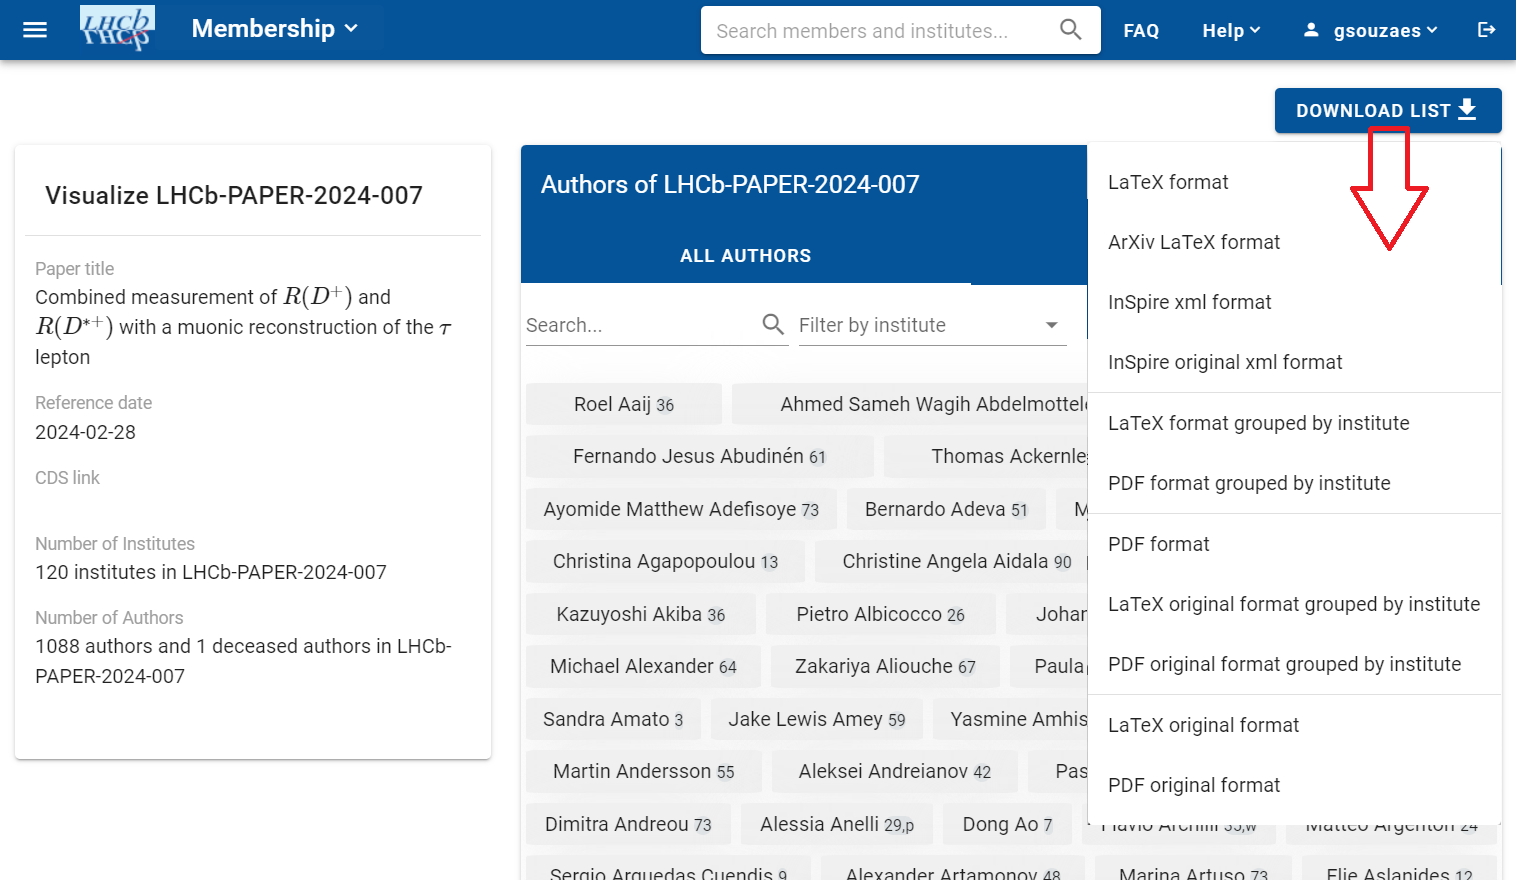
\includegraphics[width=0.8\linewidth]{figuras/manager_paper_view_tcc.png}
    \caption{Vizualize Authors List Page.}
    \label{fig:manager_paper_view_tcc}
\end{figure}

\begin{figure}[H]
    \centering
    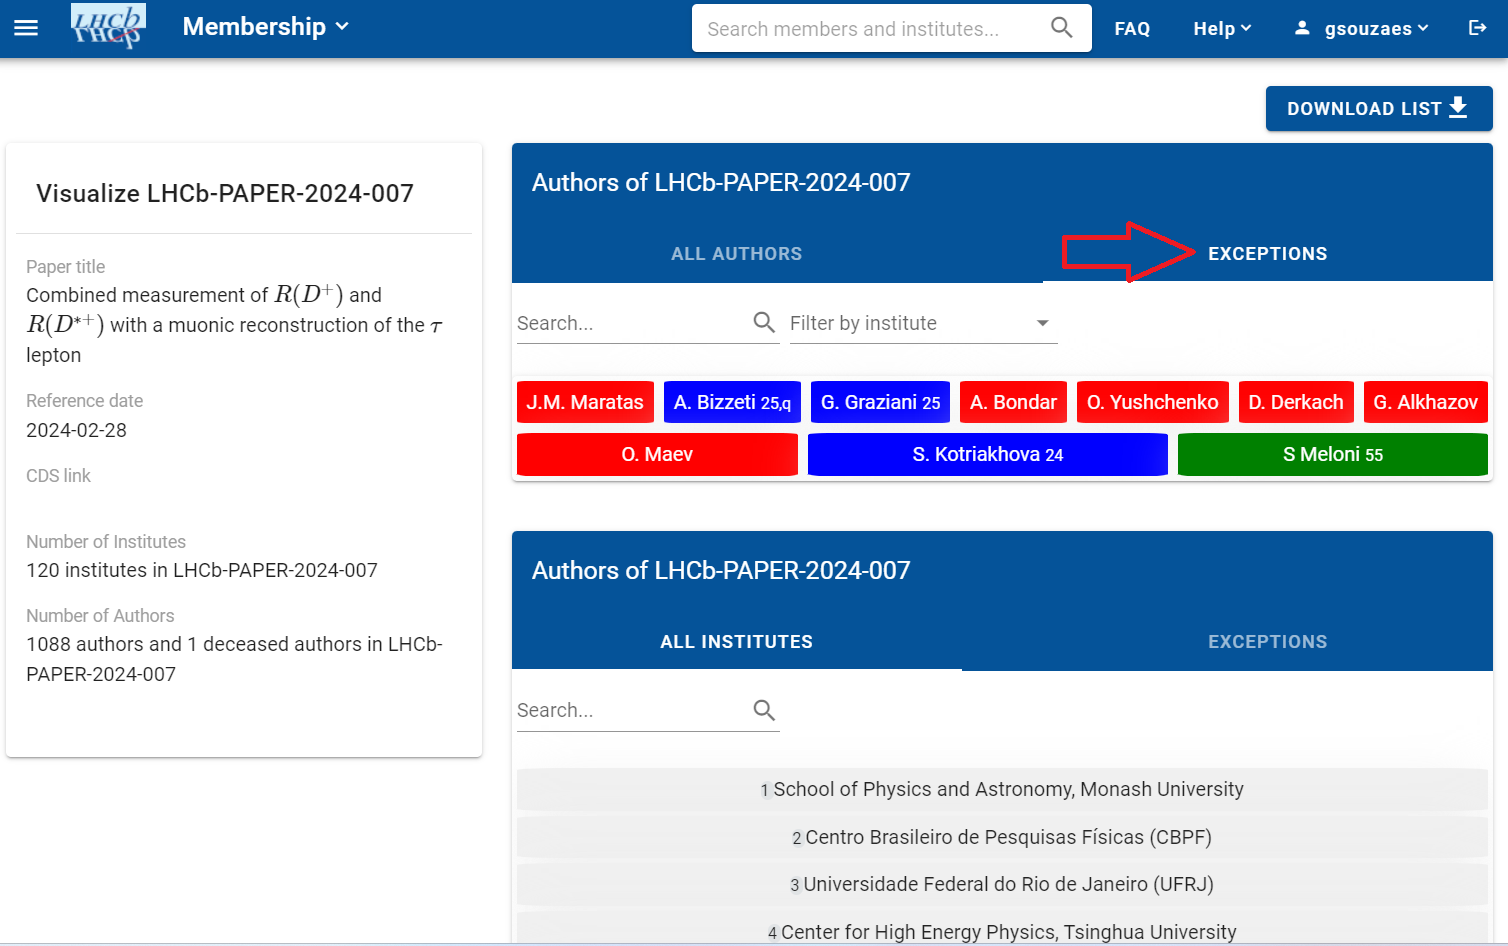
\includegraphics[width=0.8\linewidth]{figuras/authorship_exceptions_tcc.png}
    \caption{Authorship Exceptions tab.}
    \label{fig:authorship_exceptions_tcc}
\end{figure}

The two most used formats are the PDF format and the LaTeX format. This first is publicly available to expose the current list of Authors in the Collaboration and the later is usually embedded by Authors in their Papers. Figure \ref{fig:authorship_formats} displays both formats side by side. This automatic list generation is the core feature of the Authorship system, proving a reliable and standardized way for the entire Collaboration to sign a publication.

\begin{figure}[H]
    \centering
    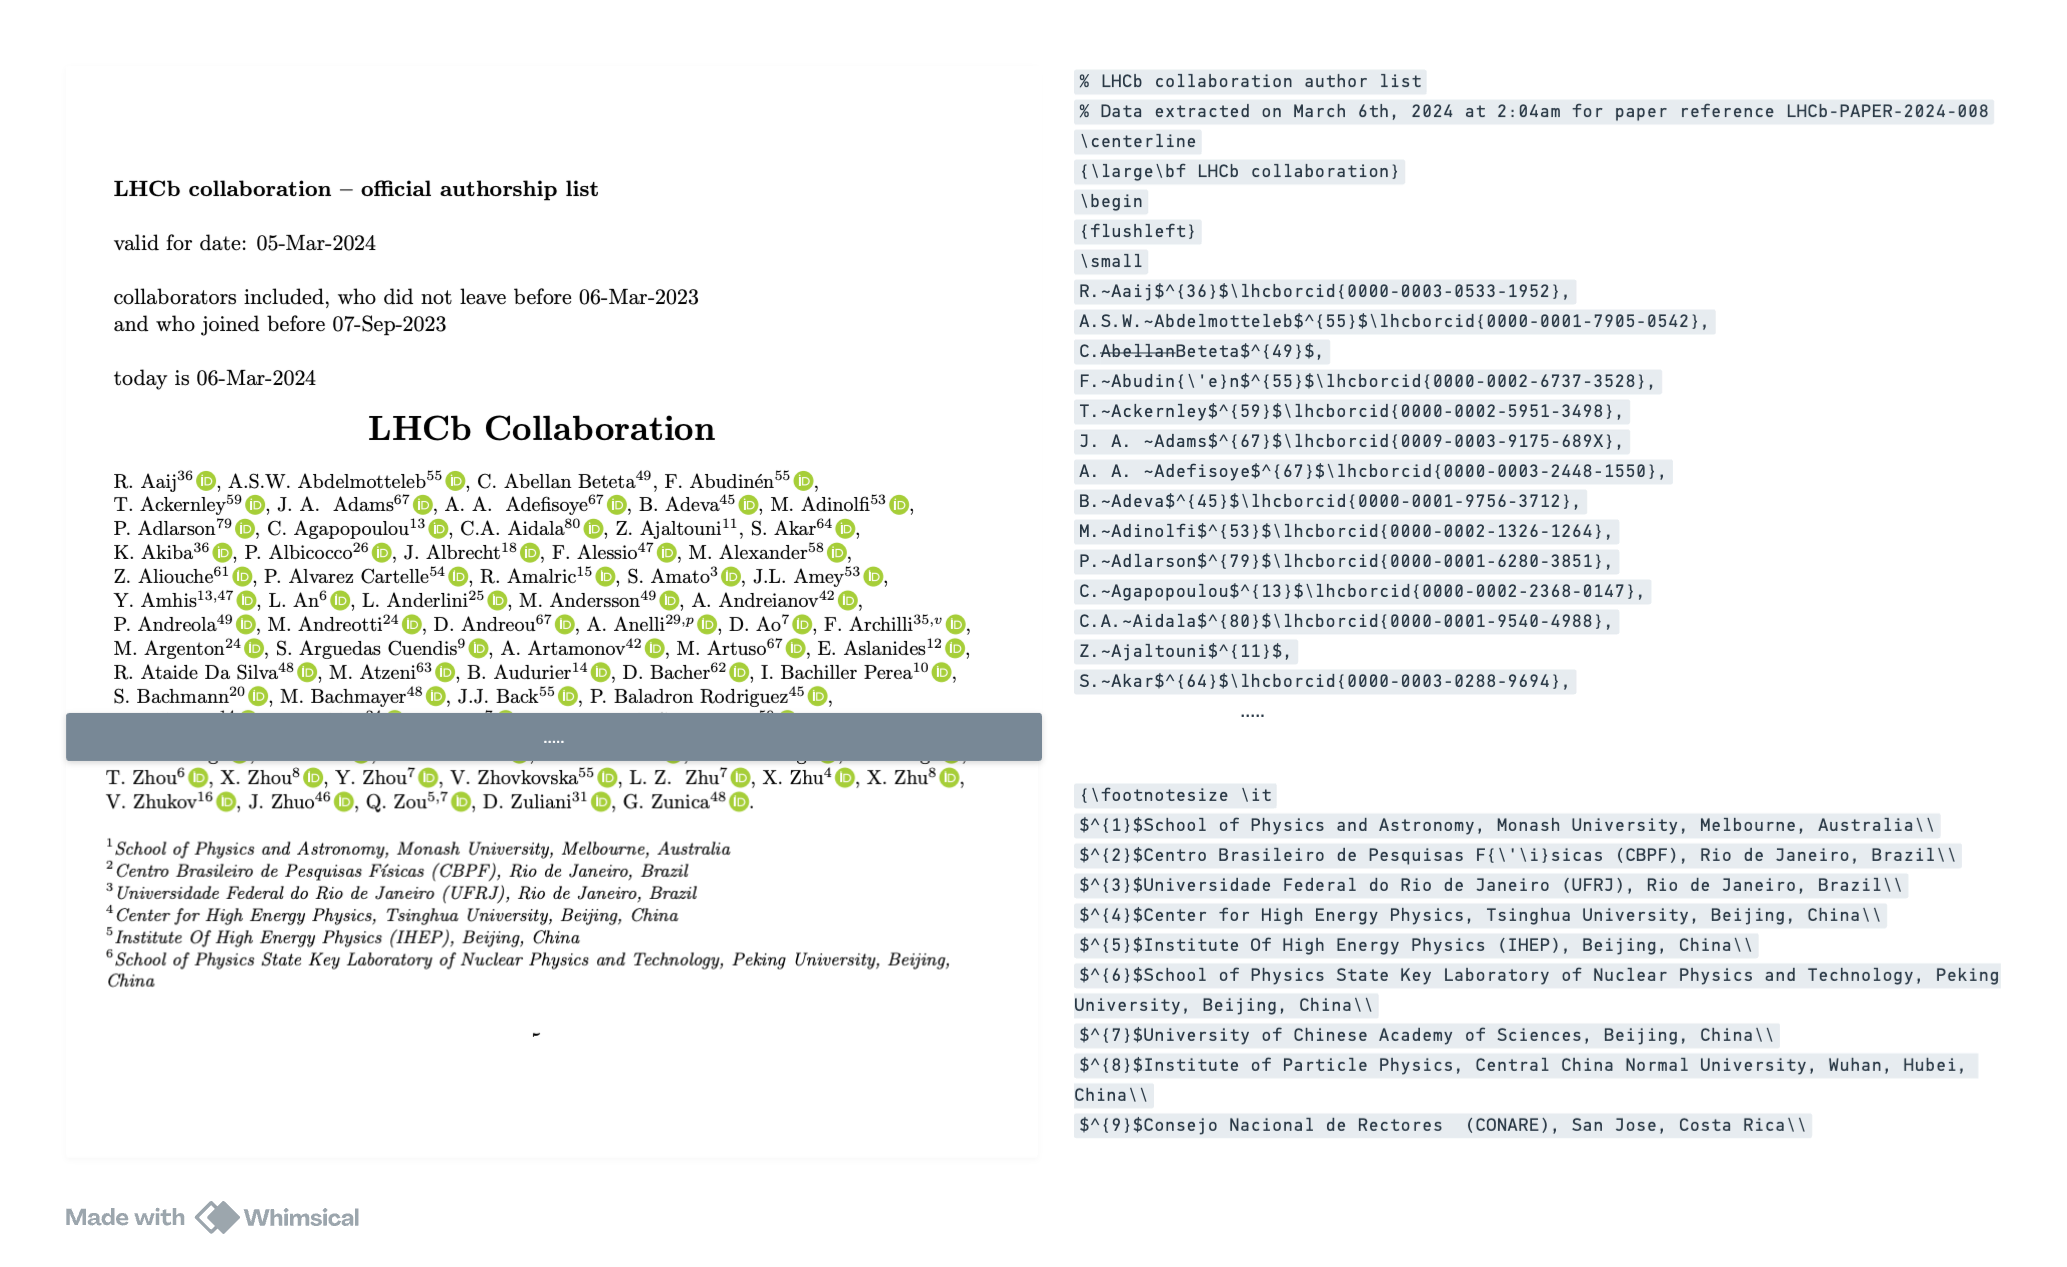
\includegraphics[width=1\linewidth]{figuras/authorship_tcc.png}
    \caption{Authorship generated files.}
    \label{fig:authorship_formats}
\end{figure}


\section{Search Implementation}  
\paragraph{} The Search Library was implemented as two different packages: a backend library for creating the search endpoints and a frontend one to provide the necessary components to build advanced search interfaces.

\subsection{Backend: search-service}

\paragraph{} The backend library is organized similarly to the backend of the Authorship web application. It also follows the Hexagonal Architecture as made explicit by the directory structure, with a Domain including classes with the knowledge to convert themselves to a piece of a SQL query.

\dirtree{%
.1 .
.2 README.md.
.2 composer.json.
.2 configuration-example.json.
.2 src.
.3 Application.
.4 DeleteSearch.
.5 DeleteSearchRepositoryInterface.php.
.4 GetSearchDetails.
.5 SearchViewRepositoryInterface.php.
.4 RunSearchWithFilters.
.5 RunSearchHandler.php.
.5 SearchInputDTO.php.
.4 SaveSearch.
.5 SaveSearchCommand.php.
.3 Domain.
.4 Conjunction.php.
.4 Exception.
.5 InvalidConfiguration.php.
.4 Field.php.
.4 Filter.php.
.4 GroupingMark.php.
.4 Operator.php.
.4 SearchConfiguration.php.
.4 SearchRepositoryInterface.php.
.4 Statement.php.
.4 Value.php.
.3 Filter.
.4 Operator.php.
.4 QueryCompilerToSQL.php.
.4 Statement.php.
.3 Infrastructure.
.4 Persistence.
.5 SqlSearchRepository.php.
.4 Provider.
.5 SearchProvider.php.
.5 SearchProviderFactory.php.
}

\paragraph{} The class \verb|Filter.php|, within the namespace \verb|LHCb\Search\Domain|, is designed for processing search query strings into SQL filter strings. This transformation involves breaking down the query into components suitable for SQL querying.

\paragraph{} The core functionality of this class is the \verb|toSqlString| method. It is responsible for converting the query string into a SQL filter string through multiple steps. Initially, spaces within Fields and Values, encapsulated by double quotes, are encoded by the \verb|encodeFieldAndValueSpaces| method with a custom encoding symbol (\verb|__|) to maintain their integrity throughout processing. Subsequently, the query string is tokenized into individual components based on spaces. Each token is then analyzed to determine its type, such as Field, Operator, Value, Grouping Maker, or Conjunction, and compiled into the corresponding SQL string component. In cases where a token is identified as an Operator, the algorithm verifies the existence of adjacent tokens to confirm a valid Field-Operator-Value sequence, throwing an \verb|InvalidArgumentException| if either is absent. The components are then synthesized into an SQL statement utilizing configuration settings and a \verb|Statement| object. Tokens identified as Grouping Marks or Conjunctions are directly translated to their SQL counterparts. The assembly of these components results in a single string, with spaces previously encoded as \verb|__| being reverted to actual spaces. The process concludes with the SQL string being encapsulated within a WHERE clause, surrounded by parentheses, or returning an empty string if the query yields no result.

\paragraph{} The \verb|encodeFieldAndValueSpaces| is dedicated to encoding spaces within Fields and Values with the special marker (\verb|__|) to differentiate them from delimiter spaces in the query string. This encoding is achieved by scanning the input string character by character, replacing spaces with the custom encoding upon encountering a double quote until its corresponding closing double quote is identified. The outcome is a string devoid of double quotes and with spaces condensed to a singular form.

\paragraph{} The pseudo-code outlined in listing \ref{lst:query} delineates the sequence of transformations applied to a query string input. Notably, the \verb|$customMatch| parameter is employed in intricate scenarios requiring the injection of a custom WHERE clause component. This necessity arises when the relevant data resides in a different table from the one targeted by the query execution. 

\begin{lstlisting}[language=PHP, caption={Transformations to the query string input.}, label=lst:query]
$queryString = "responsibleInstitutes" contain "Universidade de Santiago de Compostela"
...
$queryString = "responsibleInstitutes" contain "Universidade__de__Santiago__de__Compostela"
...
$tokens = ["responsibleInstitutes", "contain", "Universidade__de__Santiago__de__Compostela"]
...
new Statement(
    new Field("RESPONSIBLE_INSTITUTE_NAMES", "string", null),
    new Operator("contain"),
    new Value("Universidade de Santiago de Compostela", "string", null),
    $customMatch
);
...
$sqlWhereClause = "RESPONSIBLE_INSTITUTE_NAMES LIKE '%Universidade de Santiago de Compostela%'"
\end{lstlisting}

\noindent
Once the \verb|$sqlWhereClause| is defined, it is applied to a base query and executed on the search-service-dependent application database. The mapping from the field \verb|responsibleInstitutes| to the column \verb|RESPONSIBLE_INSTITUTE_NAMES| is defined on a JSON configuration file provided to the library by the application using it.


\paragraph{} The frontend search library enables a variety of customizable settings, including reordering and hiding columns, sorting information, changing pagination settings, and more. These customizations are reflected in the Vuex JSON object that represents the interface state. This state can be saved and later retrieved through the use of the \verb|SaveSearchCommand|, which is utilized by the \verb|SearchProvider| to persist the frontend state in the database. The saved states can then be consulted or deleted.

\paragraph{} To expose search endpoints, a dependent application must create a JSON configuration file. This file should include the base query path (listing \ref{lst:search_config}, line 2), the lookup view name, primary key, and the primary key of the entity table. Additionally, the file must contain mappings for each available Search Field. In the mapping settings, it is required to define the properties \texttt{type}, \texttt{column} (the column name in the select query), and \texttt{compatibleOperators}. For datetime fields, specifying the expected format is optional; if unspecified, the system defaults to casting both the column date and the query string input date to the ISO 8601 yyyy-MM-dd'T'HH:mm:ss format \cite{iso8601wikipedia}. The configuration also accommodates complex matches where data is not in the Entity table, necessitating a JOIN to include necessary columns for the WHERE clause. This is addressed by the \texttt{customMatch} option shown in listing \ref{lst:search_config} line 23, enabling developers to inject a custom subquery into the WHERE clause in which the Search Value will be injected replacing the \texttt{\_\_VALUE\_\_} macro. A common use of \texttt{customMatch} is to verify if the main Entity ID exists within a specific linking table.

\begin{lstlisting}[language=json, caption={Search configuration example.}, basicstyle=\tiny, label=lst:search_config]
{
    "query": "resources/queries/select/institute-search.sql",
    "lookup": {
        "lookupTable": "INSTITUTE_LOOKUP_VIEW",
        "lookupTablePK": "ID",
        "mainTablePK": "\"id\""
    },
    "id": {
        "compatibleOperators": ["=", "!="],
        "column": "ID"
    },
    "latexName": {
        "compatibleOperators": ["contain", "not-contain", "=", "!="],
        "colum.n": "LAST_NAME_LATEX"
    },
    "responsiblePersons": {
        "type": "string",
        "compatibleOperators": ["contain", "not-contain", "=", "!="],
        "column": "\"responsiblePersons\"",
        "customMatch": [
            {
                "operator": "contain",
                "match": "\"id\" IN (SELECT INSTITUTE_ID FROM GL_ENTITY_RESPONSIBLE WHERE RESPONSIBLE_ID = __VALUE__)"
            },
            ...
        ]
    },
    "modifiedOn": {
        "type": "date",
        "format": "YYYY-MM-DD",
        "compatibleOperators": [">", "<", ">=", "<=", "="],
        "column": "MODIFIED_ON"
    },
    ...
}
\end{lstlisting}

\paragraph{} The query mentioned in listing \ref{lst:search_config}, line 2, appears in snippet \ref{lst:search_queries}. This snippet also includes the lookup view, which consists of an ID column and a second column that concatenates all columns utilized in the base query.

\begin{lstlisting}[language=SQL, caption={Base Query and Lookup View.}, basicstyle=\tiny, label=lst:search_queries]
-- Base Query
SELECT
ID as "id",
NAME as "name",
LATEX_NAME as "latexName",
RESPONSIBLE_IDS as "responsiblePersons",
INSPIRE_NAME as "inspireName",
ENGLISH_NAME as "englishName",
MNE_CODE as "mnemonicCode",
WEBPAGE as "webpage",
TO_CHAR(MODIFIED_ON, 'yyyy-mm-dd') as "modifiedOn"
...
FROM INSTITUTE_VIEW

-- Lookup view
create view INSTITUTE_LOOKUP_VIEW as
SELECT
    i.ID,
    I.NAME || I.LATEX_NAME || TO_CHAR(I.MODIFIED_ON, 'YYYY-MM-DD')
    || I.RESPONSIBLE_IDS || I.INSPIRE_NAME || I.ENGLISH_NAME || 
    I.MNE_CODE || I.WEBPAGE ... AS lookup
    FROM
        INSTITUTE_VIEW i
\end{lstlisting}

\paragraph{} Finally, the dependent application must define a Controller method that receives the request parameters, instantiates a \verb|SearchInputDTO|, and calls the \verb|runSearch| method, passing the DTO and the path to the search configuration JSON file. The \texttt{SearchInputDTO} accepts the following parameters: \verb|$offset| (used for pagination; for instance, if there is a result set of 200 records and the offset value is 50, the first 50 records will not appear in the response), \verb|$limit| (used to limit the number of records in the response), \verb|$sortByField| (the search field used to sort the results), \texttt{\$sortDesc} (determines if sorting is in ascending or descending order), \verb|$lookupText| (text input used to further filter the results), and \verb|$queryString| (string parsed into the WHERE clause). The search results are always provided in a JSON format consisting of flat objects, as exemplified in the API response shown on listing \ref{lst:search_results}. The \verb|SearchProvider| exposes the concrete implementation of all use cases, and the \verb|SearchProviderFactory|, which takes the database credentials as input, instantiates a \verb|SearchProvider|, resolving all its dependencies


\begin{lstlisting}[language=php, caption={InstituteController's search method.}, basicstyle=\tiny, label=lst:search_controller]
public function search(Api $api) {
    $responseBody = null;
    $input = $api->getRequest()->getParameters();
    $searchParameters = new SearchInputDTO($input);
    try {
        $responseBody = json_encode(
            $this->searchProvider->runSearch(
                $searchParameters,
                __DIR__ . "/../../../../resources/search/institute.json"
            )
        );
    } catch (\InvalidArgumentException $e) {
        $this->throwForbiddenException($e->getMessage());
    }
    $response = $api->getResponse();
    $response->getBody()->write($responseBody);
    return $response->withHeader("content-type", "application/json");
}
\end{lstlisting}

\begin{lstlisting}[language=json, caption={Search output example.}, basicstyle=\tiny, label=lst:search_results]
{
  "results": [
    {
        "id": "2",
        "name": "Universidade Federal  do Rio de Janeiro (UFRJ)",
        "latexName": "Universidade Federal do Rio de Janeiro (UFRJ)",
        "responsiblePersons": "1;2;3",
        "inspireName": "Rio de Janeiro Federal U.",
        "englishName": "Federal University of  Rio de Janeiro (UFRJ)",
        "mnemonicCode": "RIO",
        "webpage": "www.if.ufrj.br",
        ...
        "modifiedOn": "2007-05-11"
    },
    {
        "id": "1",
        "name": "CBPF - Centro Brasileiro de   Pesquisas Fisicas (CBPF)",
        "latexName": "Centro Brasileiro de Pesquisas F{\\'\\i}sicas (CBPF)",
        "responsiblePersons": "4;5;6",
        "inspireName": "Rio de Janeiro, CBPF",
        "englishName": "CBPF -  Brazilian Center for  Physics Research (CBPF)",
        "mnemonicCode": "CBP",
        "webpage": "www.cbpf.br",
        ...
        "modifiedOn": "2007-05-11"
    }
  ],
  "numberOfResults": "4"
}
\end{lstlisting}

\subsection{Search frontend}

\paragraph{} The search frontend components constitute the foundational elements for constructing an advanced search interface. Encapsulated within the \verb|SuperSearch| wrapper, they aim to minimize the boilerplate code required for configuring the interface. An example of an SFC template for the Institute Search interface, utilizing the SuperSearch wrapper, is illustrated in listing \ref{lst:institute_sfc_template}. This component requires a set of obligatory properties, including a \verb|table-title| and the \verb|headers|, which are JSON objects delineating the column names and their corresponding keys in the item list retrieved from the backend. Furthermore, the provision of the \verb|search-function| prop is also mandatory; it assigns the JavaScript function responsible for querying the backend API to fetch the search results. This function receives a \verb|searchParameters| argument, which the search frontend library automatically supplies. These parameters are then used to instantiate the \verb|SearchInputDTO| on the backend. Similar processes apply for the functionalities of saving, loading, and deleting search templates. The \verb|filter-options| specifies the available Search Fields within the interface, while the \verb|user| object is required for performing authorization checks. Additionally, the \verb|router| property is essential for the library to interpret the search parameters derived from the URL query string. In the template (listing \ref{lst:institute_sfc_template}, lines 17-24), the usage of slots API enables developers to customize each column by substituting the default text content with alternatives. In the script portion of the Institute Search SFC (presented on listing  \ref{lst:institute_sfc_script}), the search mixin is incorporated, granting access to the search state—including pagination parameters, the current querystring, and the presently loaded results—and providing methods to execute search operations. These operations encompass generating a new querystring based on user inputs and executing a GET request to the API. For instance, the \verb|getSearchResults| method (imported from the mixin) is invoked within the mounted hook to initiate the loading of an empty search, thereby ensuring that the process of fetching all entities starts immediately upon the user's page access.

\begin{lstlisting}[language=HTML, caption=Institute Search SFC template., label=lst:institute_sfc_template]
<template>
  <VContainer fluid>
      <SuperSearch
          table-title="Institute search"
          :headers="headers"
          :search-function="searchInstitute"
          :filter-options="filterOptions"
          :selectable-rows="false"
          :entity-details-route="'/membership/institute/details/:var_id'"
          :search-type="{id: 4, name: 'Institute search'}"
          :save-search-function="saveSearchFunction()"
          :load-searches-function="loadSearchesFunction()"
          :delete-search-function="deleteSearchFunction()"
          :user="user"
          :router="vueRouter"
      >
          <template v-slot:item.membersStatus="{ item }">
              <VChip
                  :color="membersStatusColor(item.membersStatus)"
                  small
              >
                  {{ item.membersStatus }}
              </VChip>
          </template>
          ...
      </SuperSearch>
  </VContainer>
</template>
\end{lstlisting}

\begin{lstlisting}[language=javascript, caption=Institute Search SFC script., label=lst:institute_sfc_script ]

<script>
import { mapActions, mapMutations, mapGetters } from 'vuex';
...
import searchApi from '../../api/search';

export default {
  name: 'ModelSearch',
  components: { SuperSearch },
  mixins: [searchMixin],
  data() {
      return {
          headers: [
              { text: 'Details', value: 'id', width: 70 },
              { text: 'Name', value: 'name', width: 350 },
              { text: 'Members Status', value: 'membersStatus', width: 70 },
              ...
              { text: 'Collaboration Entry Date', value: 'entryDateString', width: 110 },
              { text: 'Comments', value: 'comments', width: 500 },
          ],
          filterOptions: [
              {
                  name: 'Id', value: 'id', operators: ['equals', 'different from'], type: 'VTextField',
              },
              {
                  name: 'Name', value: 'name', operators: ['contains', 'does not contain', 'equals', 'different from'], type: 'VTextField',
              },
              {
                  name: 'Members Status',
                  value: 'membersStatus',
                  operators: ['equals', 'different from'],
                  type: 'VAutocomplete',
                  items: [{ name: 'Active' }, { name: 'Inactive' }, { name: 'Upcoming' }],
                  optionName: 'name',
                  optionValue: 'name',
              },
              ...
              {
                  name: 'Collaboration Entry Date', value: 'entryDate', operators: ['equals', 'greater or equals', 'less or equals', 'greater than', 'less than', 'different from'], type: 'Date',
              },
              {
                  name: 'Comments', value: 'comments', operators: ['contains', 'does not contain', 'is empty', 'is not empty'], type: 'VTextfield',
              },
          ],
          greybookLink: 'https://greybook.cern.ch/greybook/institute/detail?id=',
          exception: {
              jiraLink: process.env.VUE_APP_JIRA_LINK,
              errorMessage: null,
          },
      };
  },
  computed: {
      ...mapGetters('user', [
          'user',
      ]),
      vueRouter() {
          return this.$router;
      },
  },
  mounted() {
      this.getSearchResults();
  },
  methods: {
      ...mapActions('search', ['getSearchResults']),
      ...mapActions('institute', ['searchInstitute', 'fetchAllInstitutes']),
      ...mapMutations('exception', ['activeException']),
      saveSearchFunction: () => searchApi.saveSearch,
      loadSearchesFunction: () => searchApi.loadSearches,
      deleteSearchFunction: () => searchApi.deleteSearch,
      membersStatusColor(membersStatus) {
          switch (membersStatus) {
              case 'Active':
                  return 'success';
              case 'Inactive':
                  return 'error';
              default:
                  return 'primary';
          }
      },
  },
};

</script>
\end{lstlisting}

\paragraph{} As illustrated in Figure \ref{fig:search_components}, every search component encapsulated within the \verb|SuperSearch| demonstrates the system's modular design. This flexibility allows developers to craft distinct data visualization interfaces, catering to scenarios where an advanced search interface may be unnecessarily complex. Within the Membership system, a specific requirement exists to categorize institutes based on their Participation Type. While the Institute Search page could serve this purpose, a more intuitive solution involves a table accompanied by a dropdown list enumerating all Participation Types. Upon selection, the system dynamically populates the table with Institutes corresponding to the chosen type, as depicted in Figure \ref{fig:simple_search}. This simplification is achieved by replacing the advanced search components via the Slots API and incorporating a select input. The input modification triggers a change in the \verb|searchValue|, leading to the generation of a new query string: 
\verb|"participationStatus" = "active"|

\verb|AND "participationStatusId" = "${this.searchValue}"|. 

\noindent
This query string, along with additional search parameters, is dispatched to the backend API for processing. The API, in turn, retrieves the pertinent data to populate the table with the results.

\begin{figure}[H]
    \centering
    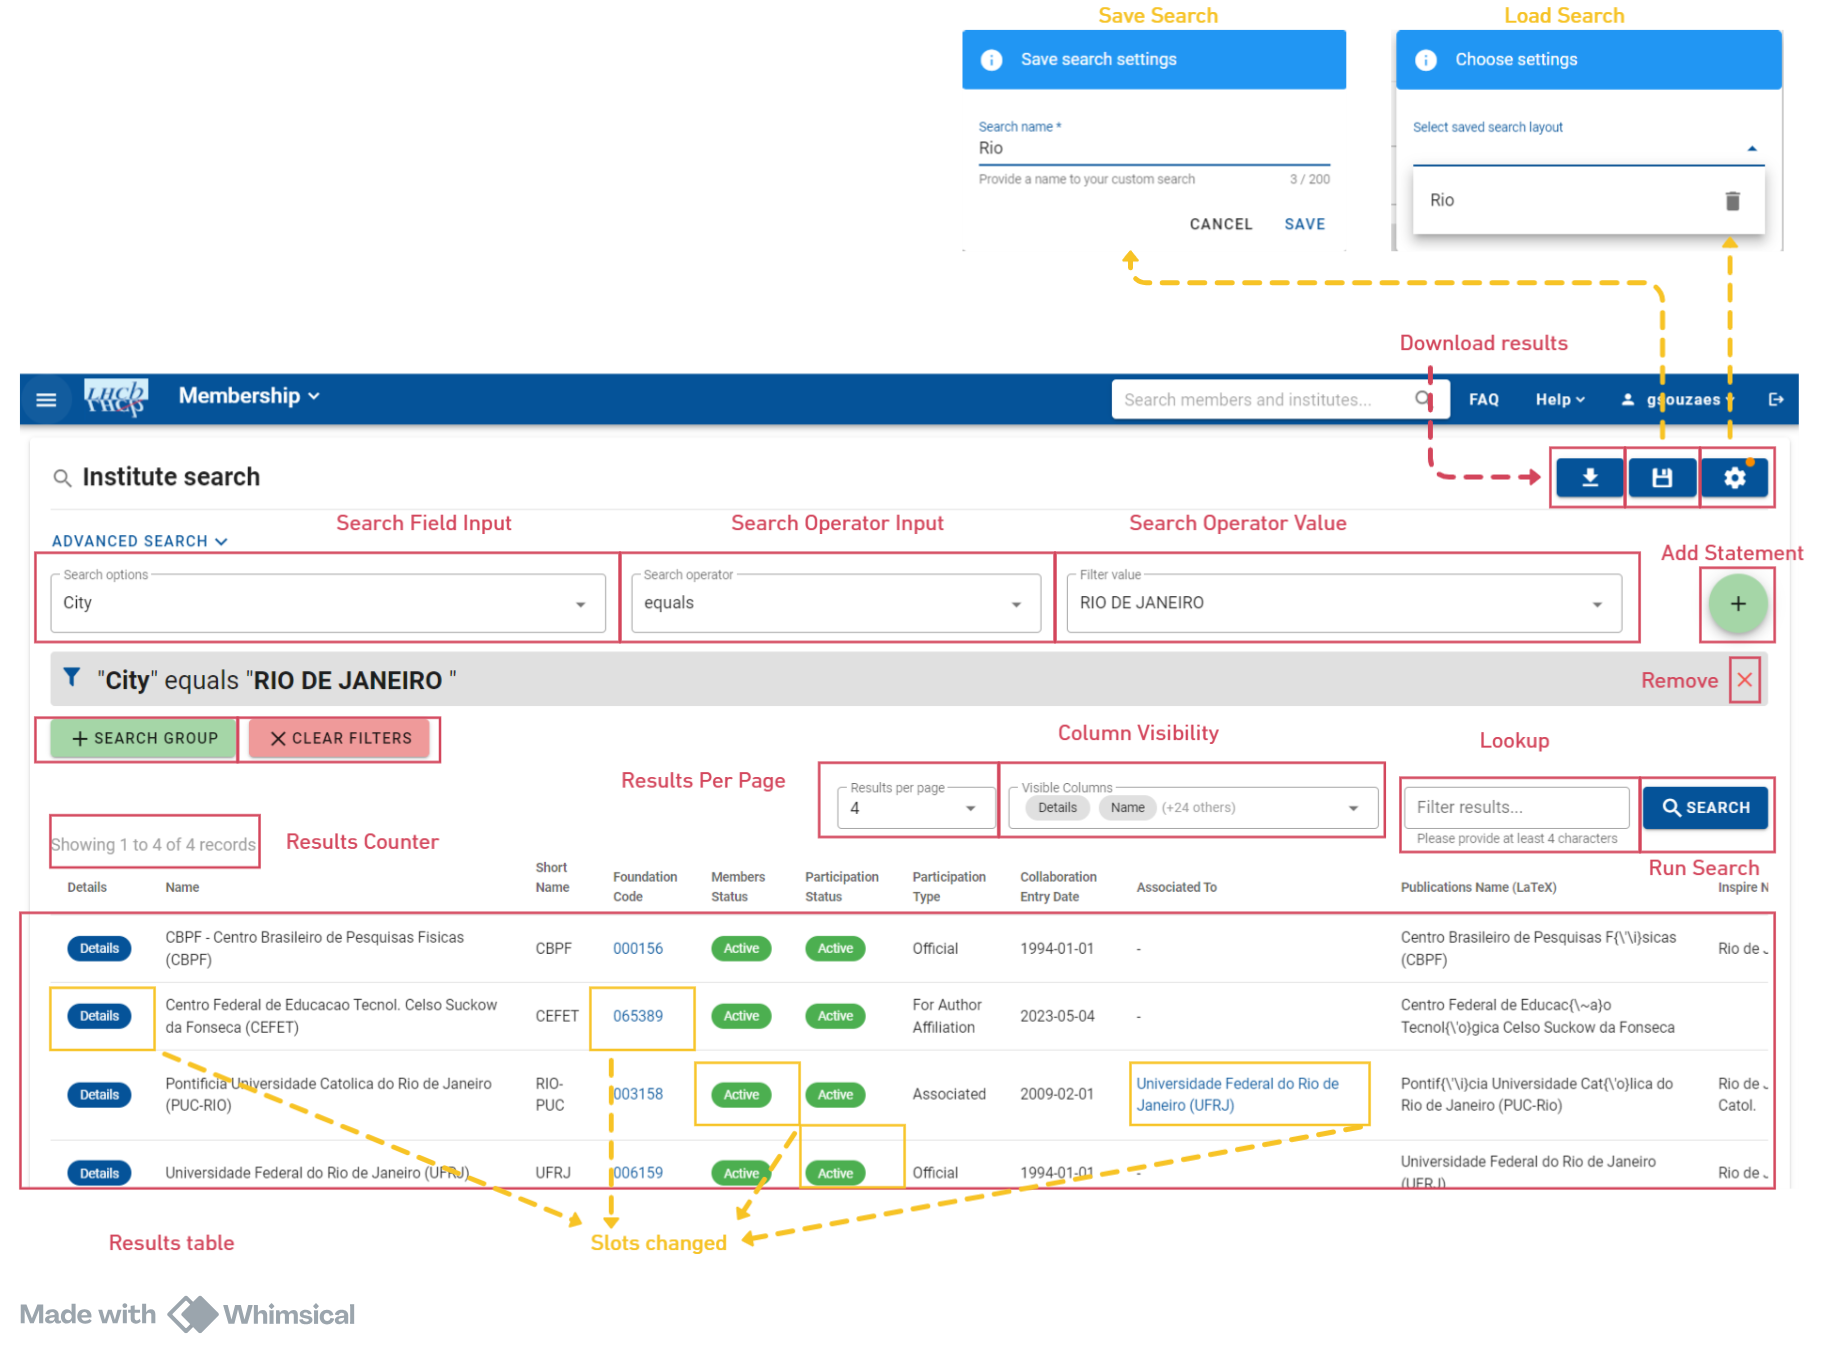
\includegraphics[width=1.0\linewidth]{figuras/search_components_marked.png}
    \caption{Institute Search Components.}
    \label{fig:search_components}
\end{figure}

\begin{figure} [H]
    \centering
    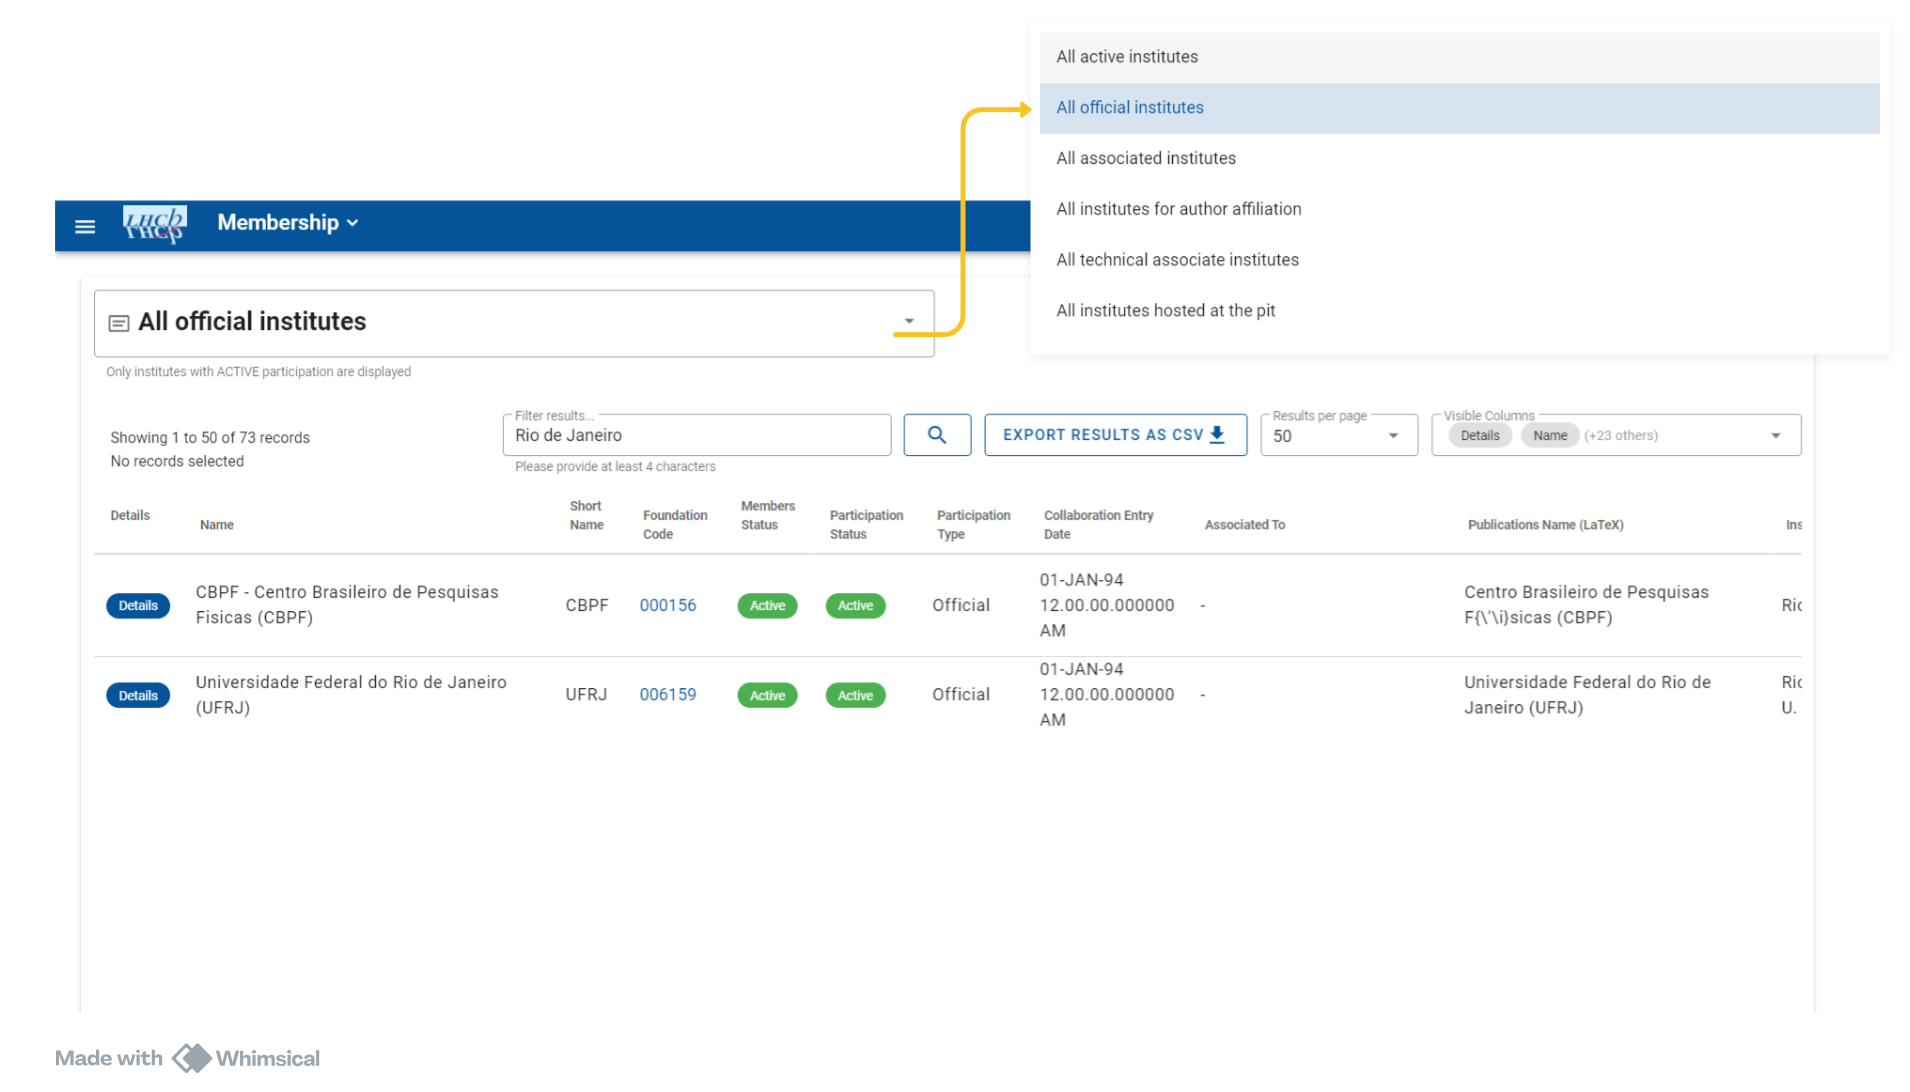
\includegraphics[width=1\linewidth]{figuras/simple_search.png}
    \caption{Simpler search visualization to list all Institutes according to their Participation Type.}
    \label{fig:simple_search}
\end{figure}

\section{Membership Implementation} 

\paragraph{} The implementation of the Membership system occurred within a period when the Hexagonal Architecture was firmly established as the chosen design paradigm for the Glance systems. Consequently, the Membership system does not exhibit a heterogeneous architectural approach similar to that of the Authorship system. The implementation provided the same existing functionalities and mostly improved use cases that benefit from the new Super Search and introduced approval workflows and interfaces with graphs.

\subsection{The Membership Architecture}

\paragraph{} It was established by the team that the Membership system would encompass the Authorship system and proceed to integrate the additional functionalities within the same application, as Authorship inherently falls within the purview of the Membership system's responsibilities. Unlike the singular context termed \verb|Authorship| within the Authorship system, the Membership system encompasses multiple requirements that do not uniformly align within a single domain. Here, the concept of Bounded Context (BC) as described on \cite{fowler2014bounded} significantly enhances the structural organization of the application. Bounded Context strategically addresses the complexities of large models and team coordination by partitioning a system into distinct segments, each characterized by its cohesive domain. This methodology not only facilitates a clearer segmentation of the system's components but also enhances team communication and understanding. Central to DDD is the creation of software that accurately reflects the domain's foundational models, fostering a shared language between developers and domain experts. This shared or Ubiquitous Language ensures consistency within a Bounded Context, while also acknowledging the impracticality of a singular model spanning a vast system. DDD advocates for the division of the system into Bounded Contexts, each with a model that maintains internal consistency yet may diverge from others, particularly concerning common concepts such as Members. An LHCb Member in the \verb|Member| context/namespace contains all the registration information the collaboration stores for its members, including the profile picture, list of Appointments, Employment, and more. A Member in the \verb|Authorship| context, on the other hand, is an Author and only contains the required information for authorship purposes. Communication between Bounded Contexts is done using the Classes from the Application Layer (Handlers and Repository Interfaces) which can have dependencies from Application-layer classes of a different BC. Inside the same BC, dependencies still point inwards (Infrastructure classes depend on Application-layer classes, which depend on Domain classes).


\paragraph{} The Modular Monolith concept is relatively recent in the Software Engineering literature. Ruoyu Su and Xiaozhou Li conducted a literature review on \cite{su2024modular} and defined a Modular Monolith as ``a software architecture pattern that strategically combines the simplicity of a monolithic structure with the advantages of microservices. In this approach, the system is organized into loosely coupled modules, each delineating well-defined boundaries and explicit dependencies on other modules." This definition is similar to the classical Monolith definition because it still envisages the application as a single deployable unit, ensuring simplicity in deployment and operation management (as it is not necessary to ensure compatibility of different service versions such as in microservices). However, it differs in that it emphasizes modularity, loose coupling, and independence within the application's internal structure, promoting ease of development, testing, and potential for scaling specific parts of the application without the need to scale everything. Loose coupling is achieved by defining clear dependencies between the modules through interface contracts. Another major difference between the classical monolithic application and a Modular Monolith is that the latter tends to incentivize code organization based on different Domains instead of class type (Controller, Model, Repository, etc.) as described in Shopify's engineering article \cite{ShopifyModularMonoly}. In the Membership context, each Bounded Context can be seen as an independent module, with its own domain definitions and the dependencies between modules modules occur through the Application layer in module's use cases are exposed. Figure \ref{fig:membership_bc} illustrates the Membership as a Modular Monolith. Each module has its own namespace in the application.

%\paragraph{} As described in Shopify's engineering article \cite{ShopifyModularMonoly}, a modular monolith architecture involves structuring a single codebase into well-defined, independent modules. Each module represents a specific business domain or functionality but is part of the same application and deployment unit. This approach maintains the simplicity of deployment and operational characteristics of a monolith while encapsulating business logic within clear boundaries, similar to microservices. Modular monoliths aim to balance the rapid development and deployment benefits of a monolithic architecture with the flexibility and scalability often associated with microservices. By defining strict boundaries around modules, a modular monolith can prevent the common pitfalls of traditional monolithic applications, such as tight coupling and complexity, making the system more maintainable and scalable within the confines of a single codebase. By introducing Bounded Contexts and decoupling the frontend and backend code, the Membership system was developed as a Modular Monolith. Figure \ref{fig:membership_bc} represents visually some of the Membership BCs.

\begin{figure}[H]
    \centering
    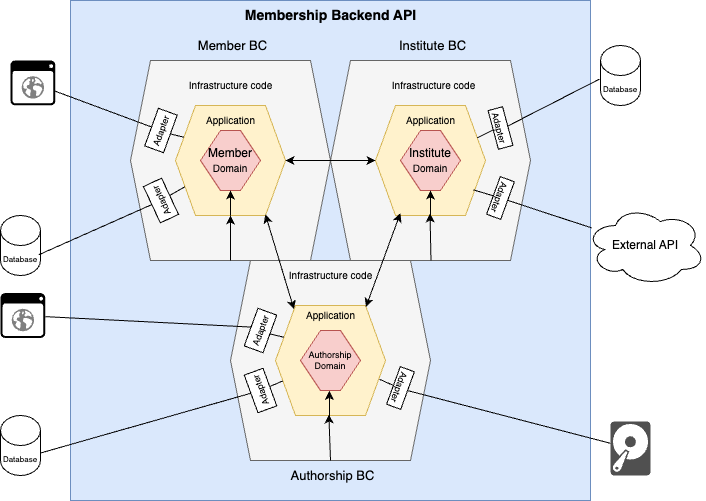
\includegraphics[width=1\linewidth]{figuras/modular_monolith (7).png}
    \caption{Membership Bounded Contexts.}
    \label{fig:membership_bc}
\end{figure}


\subsection{Workflow Tracking}

\paragraph{}Membership Version 2 introduced significant enhancements, notably in the tooling for managing internal processes via an approval workflow. The primary motivation for these developments was the newcomer registration process, as detailed in section \ref{subsec:workflow_project_cap_2}. After conducting a series of interviews with the Secretariat, the process was remodeled, as depicted in Figure \ref{fig:newcomer_wf_refactor}. A key modification is the implementation of a cron job that continually queries CERN's HR internal APIs. This automation detects newcomer registrations at CERN and initiates the LHCb registration process by creating a \verb|NewcomerRegistrationRequest|. This temporary entity encapsulates all information from CERN HR, along with additional details necessary for LHCb registration, and links to the \verb|NewcomerRequestState| entity that tracks the request's current status. The newly introduced workflow has a similar number of actions when compared to the one shown in section \ref{subsec:workflow_project_cap_2}, but its key innovation lies in automating information transfer, thereby reducing manual work. Also, by creating a multi-step approval process, it also reduces the number of incorrect information persisted in the database. In the most common scenario, newcomers submit all required information to CERN HR and provide additional details for LHCb. Assuming the accuracy of this information, the Team Leader approves the request with a simple button press, a procedure also followed by the Secretariat as exemplified in Figure \ref{fig:wf_management_page}. Notifications are automatically dispatched by the system in response to state changes, significantly reducing the volume of emails exchanged among participants. Following the implementation of the newcomer registration workflow, the use of the LHCb PDF registration form was discontinued. Each state change in the approval process required a Handler class (linked to an API endpoint called by an action button in the interface) to update the \verb|NewcomerRequestState| in response to an event (exemplified in listing \ref{lst:handle_wf}). In other words, there was no state transition function to automatically evolve the state based on an event publication. This aspect improves when workflows are modeled as automatons.

\begin{figure}[H]
    \centering
    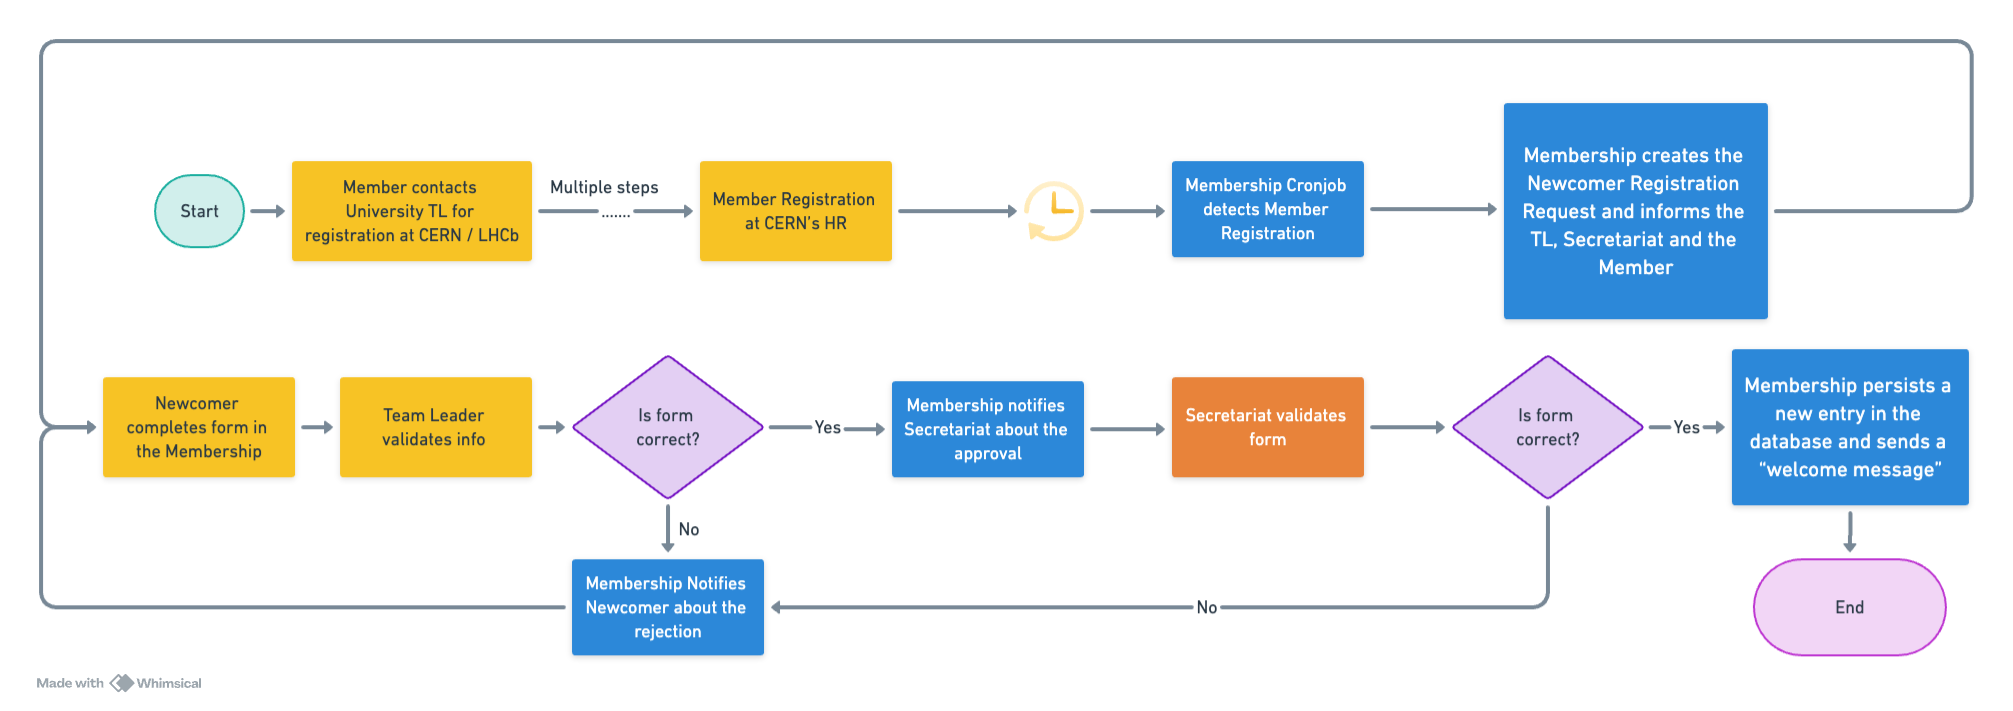
\includegraphics[width=1\linewidth]{figuras/newcomer_wf_refactor_2.png}
    \caption{Newcomer registration workflow refactored.}
    \label{fig:newcomer_wf_refactor}
\end{figure}

\begin{figure}[H]
    \centering
    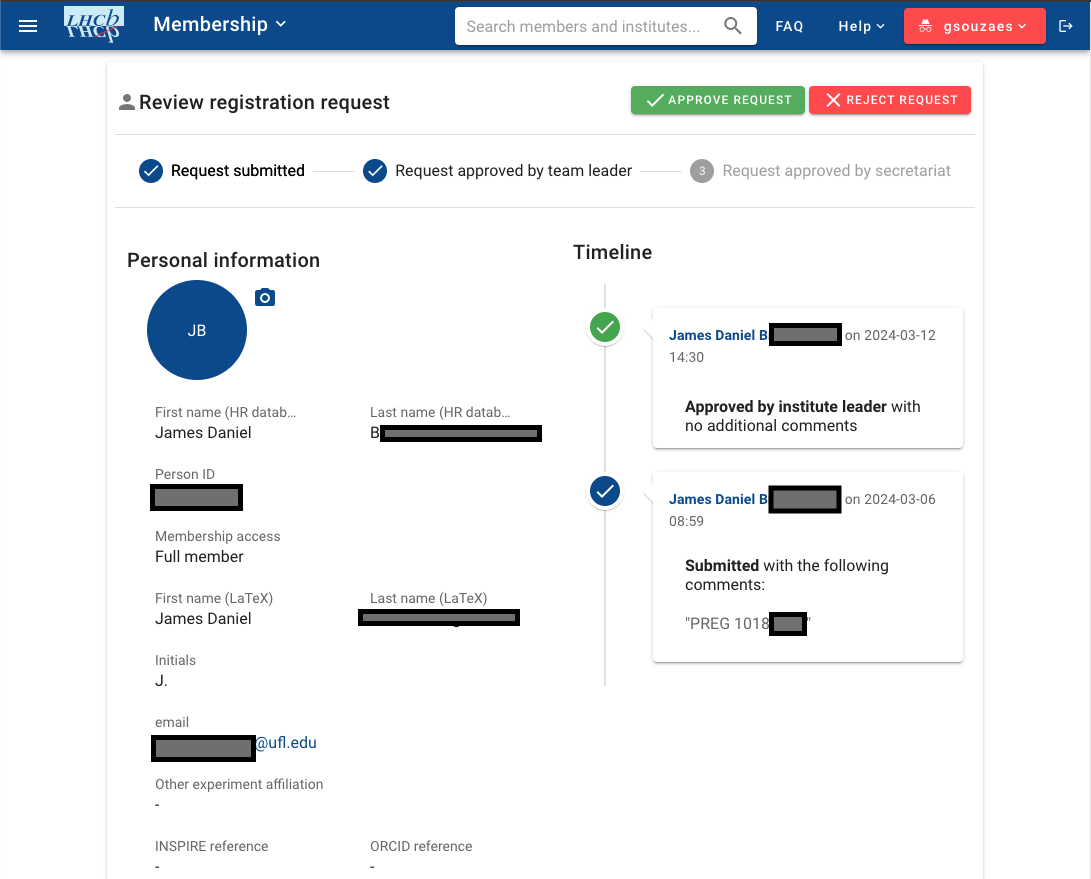
\includegraphics[width=0.65\linewidth]{figuras/wf_management_page.png}
    \caption{Newcomer Request management page pending Secretariat approval.}
    \label{fig:wf_management_page}
\end{figure}

\paragraph{} The release of the Newcomer registration workflow catalyzed the development of additional multi-step approval workflows for Members transitioning to different Institutes, altering Professions, or extending their Employments. Similar to the Newcomer registration process, these workflows were developed with a Command and Handler for each state transition (such as a button pressed on the interface to change a request to ``Rejected"), leading to a phenomenon known as class explosion. This term describes a situation where the number of classes in a system becomes excessively large as a result of attempts to accommodate every possible variation of a problem or requirement through inheritance or the creation of fine-grained classes for every piece of functionality. It was observed that the approval and rejection operations predominantly involved updating the state of the \verb|Request| entity (the possible states are shown in a state transition diagram in Figure \ref{fig:states}), as exemplified in listing \ref{lst:handle_wf}. The way to avoid these unnecessary Handlers is to model the approval workflows as automatons and introduce a state transition function that could be called from a single Handler based on events published by other parts of the system. In practice, this would mean that instead of having one API endpoint for each action button (buttons to approve a request, reject a request, and submit a request) there could be one generic endpoint to post events mapped to a Handler that calls the state transition function passing the event as argument.

\paragraph{} The diagram from Figure \ref{fig:states} can be formalized using the automaton concept already explored. Let $ G=\left(X, \Sigma, f, \Gamma, x_0, X_m\right)$ be the automaton describing the approval process. Then 
$$
X=\{U, V, W, X, Y, Z\}; \Sigma=\{a, b, c, d, e, f, g, h\}
$$
For any state $x \in X$ and event $\sigma \in \Sigma$ :
$$
f(x, \sigma)= \begin{cases}V & \text { if }(x, \sigma)=(U, a) \\ T & \text { if }(x, \sigma)=(U, b) \\ W & \text { if }(x, \sigma)=(V, d) \\ T & \text { if }(x, \sigma)=(V, e) \\ V & \text { if }(x, \sigma)=(W, c) \\ T & \text { if }(x, \sigma)=(W, h) \\ Y & \text { if }(x, \sigma)=(T, f) \\ Z & \text { if }(x, \sigma)=(T, g) \\ T & \text { if }(x, \sigma)=(Y, h) \\ V & \text { if }(x, \sigma)=(Y, c) \\ x & \text { otherwise }\end{cases}
$$
$$
\Gamma(K)=\Sigma \text { for all } K \in X; x_0=U; X_m=\{Z\}
$$

\paragraph{} The same formulation applies to all the different Membership approval workflows currently available involving the Secretariat and Team Leaders. 

\paragraph{} Concurrently with the necessity to reduce the class explosion (evident by the number of classes in the directory structure in \ref{dirTree}) and the implementation of a new system for managing LHCb publication approvals, a pressing need emerged for an enhanced workflow tracking solution. This solution should effectively manage a complex graph scenario where the user specifies \textbf{two states and a sequence of events required for transitioning between these states}. The existing challenge is that previously demonstrated graphs (such as in Figure \ref{fig:states}) typically feature a single event linking two states. The proposed solution, therefore, must accommodate more intricate interactions handling multiple events within state transitions.

\begin{lstlisting}[language=php, caption={Example of handle method to deal with the press of the approve button by the TL (Team Leader).}, basicstyle=\tiny, label=lst:handle_wf]
public function handle(ApproveNewEmploymentRequestCommand $command): int
    {
        $newEmploymentRequest = $this->workflowReadRepository
            ->findNewEmploymentRequest($command->memberId());
        $instituteLeadersIds = $this->workflowReadRepository->findInstituteLeaderIds($newEmploymentRequest->instituteId());

        $newEmploymentRequest->addState(
            new WorkflowState(
                $this->workflowRepository->findNextNewEmploymentRequestStateId(),
                WorkflowState::APPROVED_BY_INSTITUTE_LEADER,
                $command->comments(),
                $command->agentId()
            ),
            $command->memberId(),
            $instituteLeadersIds
        );

        $this->workflowRepository->insertStates($newEmploymentRequest, $command->agentId());
        $this->eventDispatcher->dispatchAll($newEmploymentRequest->releaseEvents());
        return $newEmploymentRequest->id();
    }
}
\end{lstlisting}


\noindent % Prevent indentation at the beginning of the environment
\begin{minipage}{.55\linewidth}
\label{dirTree}
\dirtree{% Your directory tree structure
.1 Application.
.2 ApproveChangeInstituteRequest.
.2 ApproveChangeProfessionRequest.
.2 ApproveNewEmploymentRequest.
.2 ApproveNewcomerRequest.
.2 .....
.2 GetChangeInstituteRequestDetails.
.2 GetChangeProfessionRequestDetails.
.2 .....
.2 GetNewEmploymentRequestDetails.
.2 GetNewcomerRequestDetails.
.2 ....
.2 RejectChangeInstituteRequest.
.2 RejectChangeProfessionRequest.
.2 RejectNewEmploymentRequest.
.2 RejectNewcomerRequest.
.2 SubmitChangeInstituteRequest.
.2 SubmitChangeProfessionRequest.
.2 SubmitNewEmploymentRequest.
.2 SubmitNewcomerRequest.
}
\end{minipage}%
\hfill
\begin{minipage}{.5\linewidth}
\begin{figure}[H]
    \centering
    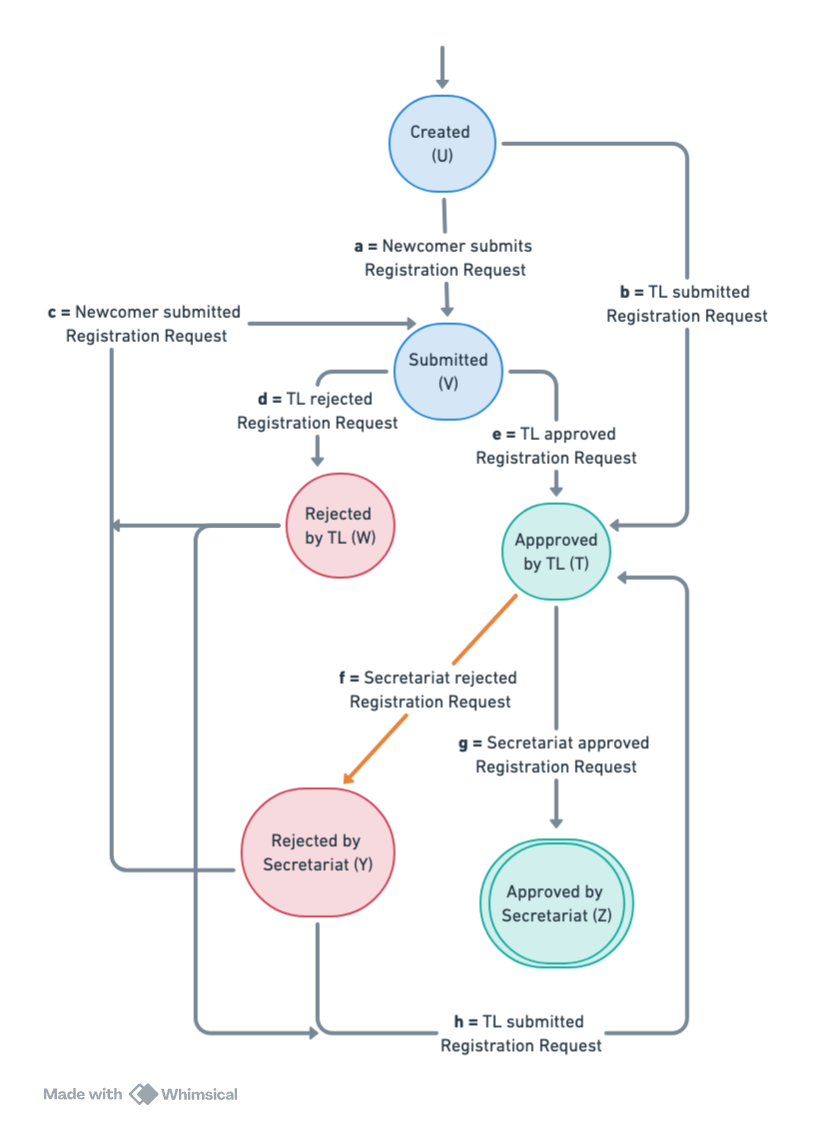
\includegraphics[width=1\linewidth]{figuras/approval_graph.png}
    \caption{Newcomer registration request graph.}
    \label{fig:states}
\end{figure}
\end{minipage}



\paragraph{} To address class explosion and minimize boilerplate code in state transitions, a new generic Workflow BC was developed. This was also inspired by the LHCb Analysis Lifecycle Management System (ALCM), which is designed around the concept of using graph theory to track the evolution and state transitions of various types of documents published by LHCb through their review procedures. The requirement for multiple events between transitions comes from ALCM, where a document usually goes to the next stage in the review process based on multiple approvals (events).

\paragraph{} In this scenario, the review stage/status is not represented as a state in a directed graph because changes are controlled by a \textbf{list} of specific events. To address this, a generic Workflow engine is introduced to manage the lifecycle of an entity. The process begins with the creation of a new Workflow class, which accepts an array of Transitions in its constructor. Each Transition consists of an initial State, a target State, an array of Events that occur in relation to the tracked entity, and an array of Conditions (analogous to events) required for a State change from the current to the target. Figure \ref{fig:abc_graph} exemplifies the registration of a Workflow with 3 States ($A$, $B$ and $C$). The instantiation of a new Workflow class is done is listing \ref{lst:figure_wf}. Transitioning from $A$ to $B$ requires the events $x$, $y$ and $z$. From $B$ to $C$ only $m$ and $n$. The automaton that describes this Workflow is $ G=(X, \Sigma, f, \Gamma, x_0, X_m)$ where
$$
X=\{A, A_1, A_2, A_3, A_4, A_5, A_6, B, B_1, B_2, C\}; \Sigma=\{x, y, z, m, n\}
$$

\noindent
Let $n_{i j}$ be the number of Conditions between State $i$ and State $j$. The number of intermediate states for each pair $(i, j)$ is $2^{n_{i j}}-2$. This indicates that the number of intermediate states grows exponentially with the number of events, emphasizing the need to register states only on demand, as demonstrated in the \verb|handleNewEvent| method in listing \ref{lst:InnerStatesGraph}.


\paragraph{} For this reason, this Workflow engine is designed in a way that intermediate states are abstracted from the user and handled internally, being only necessary to provide the initial and final States (the Stages). In the present work, a State registered by the user is also referred to as a Stage, these are the meaningful States to the final application user which must be displayed on the interface. When registering a new Workflow, the marked State will always be the current Stage in Transition without target Stage. The class shown in listing \ref{lst:InnerStatesGraph} does the processes of evolving the intermediate states and is used by the Transition class \verb|isFulfilled| method, shown in listing \ref{lst:isFulfilled}, to determine if all the Transition Conditions were satisfied. 

\paragraph{} This approach allows for the registration of all relevant \verb|State|s and \verb|Transition|s through which an Entity can progress, as exemplified in listing \ref{lst:figure_wf}.

\begin{figure} [H]
    \centering
    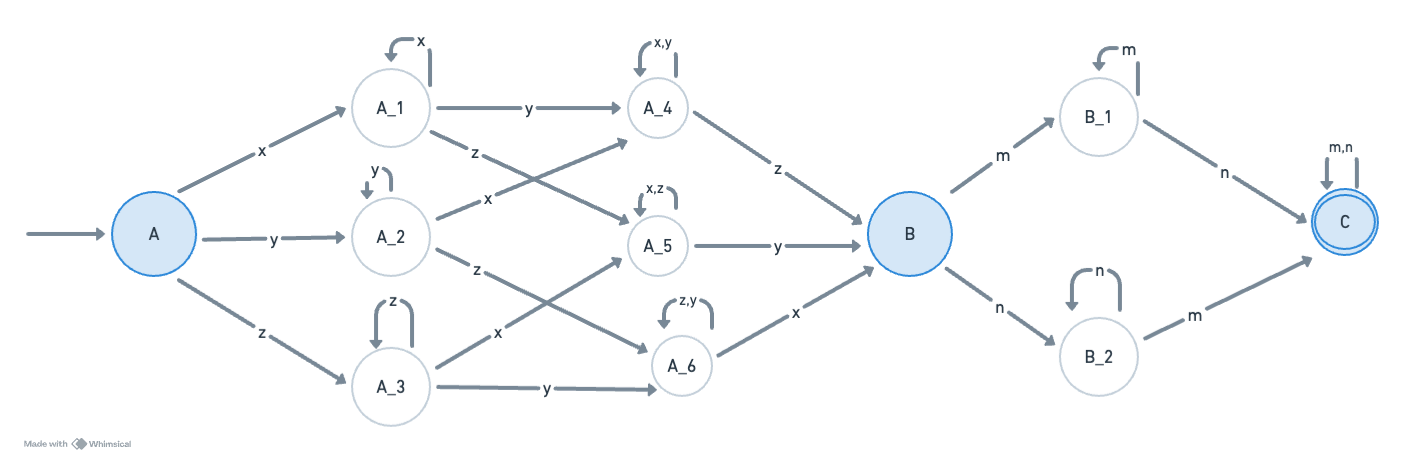
\includegraphics[width=1\linewidth]{figuras/abc_graph.png}
    \caption{Graph for three Stages $A$, $B$, and $C$. To go from $A$ to $B$, events $x$, $y$, and $z$ must occur. To go from $B$ to $C$, events $m$ and $n$ must occur. $A$, $B$, and $C$ are provided by the user and the remaining States are dynamically generated.}
    \label{fig:abc_graph}
\end{figure}

\begin{lstlisting}[language=php, caption={Workflow registration for a Figure document to be approved by the EB.}, basicstyle=\tiny, label=lst:figure_wf]
$workflow = new Workflow(
            $event->entityId(),
            FigureStage::DRAFTING,
            [
                new Transition(
                    FigureStage::DRAFTING, //current stage //A
                    FigureStage::TO_BE_REVIEWED, //next stage //B
                    [Condition::create(FigureReadyForReview::ACTION_ID, null)], //analogous to x, y, z
                    [],
                ),
                ...
                new Transition(
                    FigureStage::TO_BE_REVIEWED, // B
                    FigureStage::APPROVED, // C
                    [Condition::create(FigureApproved::ACTION_ID, null)], //analogous to m,n
                    [],
                ),
                new Transition(FigureStage::APPROVED, null, [], [],),
            ]
        );
        $this->repository->registerWorkflow($workflow, $event->agentId());
\end{lstlisting}


\begin{lstlisting}[language=php, caption={Class that handles intermediate states.}, basicstyle=\tiny, label=lst:InnerStatesGraph]
class InnerStatesGraph {
    private $states = [];
    private $events = [];
    private string $currentState;
    private string $finalState;

    public function __construct(string $initialStateName, string $finalStateName) {
        $this->currentState = $initialStateName;
        $this->finalState = $finalStateName;
        $this->states[$initialStateName] = [];
    }

    public static function fromTransition(Transition $transition): self {
        $graph = new self($transition->currentStageId(), $transition->targetStageId());
        foreach ($transition->entryConditions() as $condition) {
            $graph->addEvent($condition->actionId() . "-" . $condition->memberId());
        }
        return $graph;
    }

    public function addEvent(string $eventKey): void {
        $this->events[$eventKey] = $eventKey;
    }

    public function handleNewEvent(ActionPerformed $action): void {
        $eventKey = $action->actionId();
        if (!in_array($eventKey, $this->events)) {
            $eventKey = $eventKey . "-" . $action->agentId();
        }
        if (!in_array($eventKey, $this->events)) {
            return;
        }
        if ($this->currentState === $this->finalState) {
            return;
        }
        $currentEvents = $this->states[$this->currentState] ?? [];
        
        if (!in_array($eventKey, $currentEvents)) {
            $currentEvents[] = $eventKey;
            sort($currentEvents);
            $newStateName = implode(",", $currentEvents);
            $this->states[$newStateName] = $currentEvents;
            $this->currentState = $newStateName;
        }

        if ($this->isFinal($currentEvents)) {
            $this->currentState = $this->finalState;
        }
    }
    private function isFinal($eventsReceived): bool {
        return count($eventsReceived) === count($this->events);
    }
    public function getCurrentState() {
        return $this->currentState;
    }
\end{lstlisting}

\begin{lstlisting}[language=php, caption={Transition class isFulfilled method.}, basicstyle=\tiny, label=lst:isFulfilled]
public function isFulfilled(): bool
    {
        $graph = InnerStatesGraph::fromTransition($this);
        foreach ($this->performedActions as $action) {
            $graph->handleNewEvent($action);
        }
        return $graph->getCurrentState() == $this->targetStageId;
    }
\end{lstlisting}


%todo: talk about using the theory to validate automaton registration
%todo maybe display the code 

\paragraph{} The Workflow class implements a check to prevent the registration of lifecycles with locks. This means that if $G$ is an automaton that describes the entity lifecycle, then $\overline{L_m(G)}=L(G)$, otherwise there are locks. To perform this validation, it is not necessary to analyze any intermediate states, as those are internally handled by the system in a way that locks will not arise. To exemplify this validation, a higher-level view of the graph from Figure \ref{fig:abc_graph} is displayed in Figure \ref{fig:abc_graph_simple}. In this case the automaton $ G=(X, \Sigma, f, \Gamma, x_0, X_m)$ with
$$
X=\{A, B, C\}; \Sigma=\{v, k\}
$$
\noindent
In the given example, a visual inspection suffices to ascertain that the automaton exhibits nonblocking behavior. The \verb|HighLevelStatesGraph| class, referenced in listing \ref{lst:HighLevelStatesGraph}, computationally confirms this by identifying all viable paths originating from the initial State. The class checks the \text{no-lock condition:} \(\overline{L_m(G)}=L(G)\) by executing the following steps: First, it uses the method \verb|findAllPaths($startState)| to generate all possible paths from the initial State, which represent the generated language \(L(G)\). It then filters these paths using \verb|filterPathsEndingAtFinalState($paths)| to retain only those paths that lead to the final (marked) State, representing the marked language \(L_m(G)\). Next, the class verifies whether every path in the generated language \(L(G)\) can reach the marked State. This is done in the \verb|isNonblocking()| method, which checks if all paths found in \(L(G)\) are also present in the filtered paths leading to the final State. If there exists any path in \(L(G)\) that cannot be extended to reach the marked State, the method returns \verb|false|, indicating that \(\overline{L_m(G)} \neq L(G)\), and thus, there are locks in the system. If all paths can reach the marked State, the method returns \verb|true|, confirming \(\overline{L_m(G)} = L(G)\) and indicating a nonblocking system.



\paragraph{} This class functionality is used in the Workflow class constructor, which leverages it to validate the sequence of transitions. If a transition sequence is detected that does not comply with the nonblocking condition, the constructor raises an exception, thereby preventing the creation of a workflow that could potentially lead to a deadlock or an incomplete process execution.

\begin{figure} [H]
    \centering
    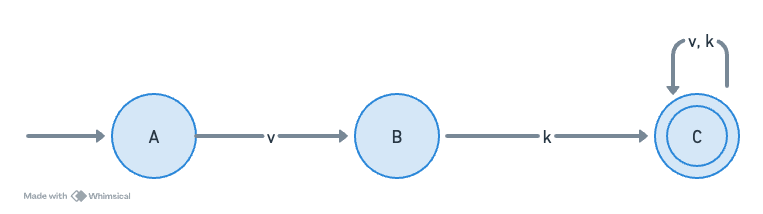
\includegraphics[width=1\linewidth]{figuras/abc_graph_simple.png}
    \caption{Graph for three Stages $A$, $B$, and $C$.}
    \label{fig:abc_graph_simple}
\end{figure}

\paragraph{} The Workflow BC provides a \verb|SaveAction| subscriber that can be invoked whenever an Event occurs to advance the State in the Entity workflow graph. \textbf{This subscriber acts as the State transition function of the system, updating the State according to an Event received.} The lifecycle will evolve through the intermediate States until all Conditions are met and a Transition from a State to a Stage occurs, indicating that the Entity State has moved to the next Stage (target State registered by the user). Through the \verb|SaveAction| subscriber, the application backend is equipped with a singular Application Use Case to post a generic Event.

\paragraph{} For Membership, this means that instead of having a unique Handler/Command pair for changing the entity State (as illustrated in listing \ref{lst:handle_wf}), a generic \verb|PostEventHandler| could be utilized for all approvals and rejections, solving the class explosion problem. This Handler would emit an Event that is captured by the \verb|SaveAction| invokable class (shown in listing \ref{lst:saveAction}). If a Transition is fulfilled (such as when the Secretariat rejects a Newcomer Request, moving it from the State \textbf{``Approved by TL"} to \textbf{``Rejected by Secretariat"} as the \textbf{``Secretariat Rejects Request"} Condition in the Transition from \textbf{``Approved by TL"} to \textbf{``Rejected by Secretariat"} is satisfied by the \textbf{``Secretariat Rejected Request"} Event. This Transaction is marked in orange in Figure \ref{fig:states}) a new Transition Fulfilled Event is dispatched. This can be monitored to, for instance, trigger a notification.

\begin{lstlisting}[language=php, caption={Workflow registration for a Figure document to be approved by the EB.}, basicstyle=\tiny, label=lst:saveAction]
final class SaveAction
{
    private $repository;
    private $eventDispatcher;
    ...
    public function __invoke(ActionPerformed $event): void
    {
        $workflow = $this->repository->findWorkflow($event->entityId());
        $workflow->recordPerformedAction($event);
        $this->repository->savePerformedAction(
            $event->entityId(),
            $event->actionId(),
            $event->agentId(),
            $event->comments()
        );

        if ($workflow->currentTransitionFulfilled()) {
            $workflow->proceed();
            $this->repository->updateWorkflowStage(
                $workflow->entityId(),
                $workflow->currentStageId(),
                $event->agentId()
            );
        }
        $this->eventDispatcher->dispatchAll($workflow->releaseEvents());
    }
}
\end{lstlisting}

\begin{lstlisting}[language=php, caption={Class to prevent blocking states.}, basicstyle=\tiny, label=lst:HighLevelStatesGraph]
class HighLevelStatesGraph {
    private $transitions = [];
    private $states = [];
    private $initialState;
    private $finalState;

    public static function fromTransitions(array $transitions, $initialState): self {
        $graph = new self($initialState);
        foreach ($transitions as $t) {
            $graph->addTransition($t->currentStageId(), $t->targetStageId());
        }
        return $graph;
    }

    public function __construct($initialState) {
        $this->initialState = $initialState;
    }

    public function addTransition($from, $to): void {
        $this->states[$from] = true;
        if ($to === null) {
            $this->finalState = $from;
        } else {
            $this->transitions[$from][] = $to;
            $this->states[$to] = true;
        }
    }

    public function isNonblocking(): bool {
        $allPaths = $this->findAllPaths($this->initialState);
        $pathsToFinal = $this->filterPathsEndingAtFinalState($allPaths);
        foreach ($allPaths as $path) {
            if (!in_array($path, $pathsToFinal)) {
                return false;
            }
        }
        return true;
    }

    public function isLocked(): bool {
        return !$this->isNonblocking();
    }

    private function findAllPaths($startState): array {
        $allPaths = [];
        $this->explorePaths($startState, [], $allPaths);
        return $allPaths;
    }

    private function explorePaths($current, $visited, &$paths, $path = ''): void {
        if (isset($visited[$current])) {
            return;
        }
        $visited[$current] = true;
        $path .= $path ? "->" . $current : $current;

        if (empty($this->transitions[$current])) {
            $paths[] = $path;
        } else {
            foreach ($this->transitions[$current] as $next) {
                $this->explorePaths($next, $visited, $paths, $path);
            }
        }
        $visited[$current] = false;
    }

    private function filterPathsEndingAtFinalState($paths): array {
        return array_filter($paths, function($path) {
            return strpos($path, $this->finalState) !== false;
        });
    }
}
\end{lstlisting}


\subsection{Features}
\paragraph{}The Membership system primarily manages the core data entities through profile pages. On a Member's profile page, LHCb Members, the Secretariat, and Team Leaders have the capability to view and update personal information. This includes changes to their publication name, profile picture, and initiating modifications to their Employment details such as Profession, Employment period, or Institute affiliation. Additionally, the system supports various other updates pertinent to a member's profile. Figure \ref{fig:member_profile} illustrates a Member's profile within the system.

\begin{figure} [H]
    \centering
    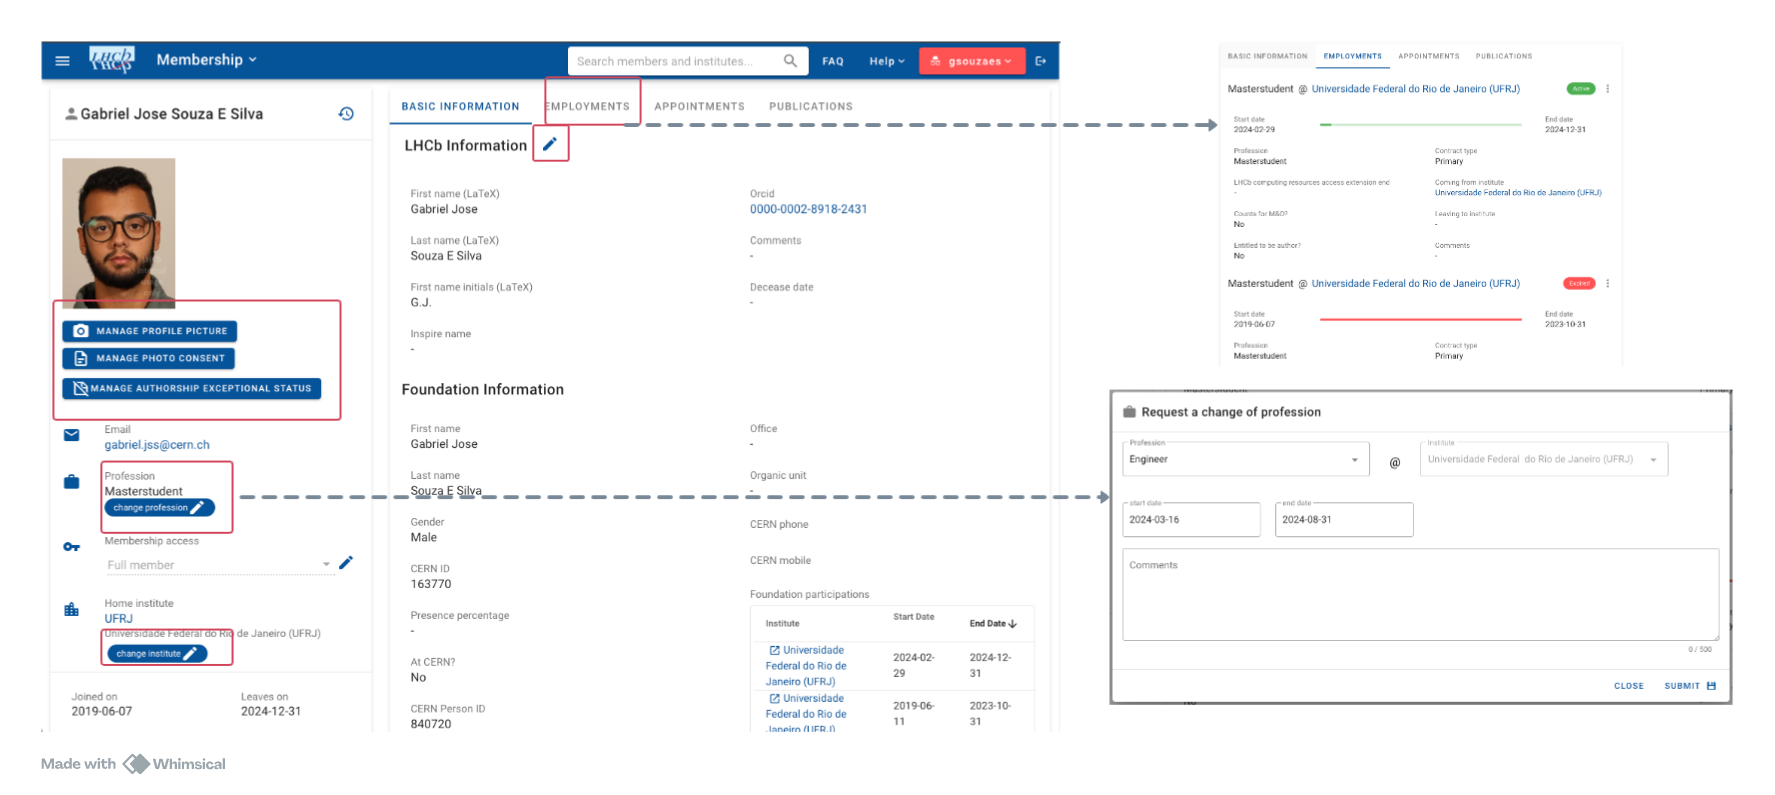
\includegraphics[width=1\linewidth]{figuras/profile.png}
    \caption{Membership Member profile.}
    \label{fig:member_profile}
\end{figure}

\paragraph{} The Institute profile page is primarily utilized by Team Leaders and Resource Coordinators for financial oversight, particularly regarding M\&O data. To facilitate access to M\&O information, an export feature is available, enabling the download of a CSV file that encapsulates the data presented on the interface. This functionality, among other user-centric enhancements, significantly augments the system's usability. Implementing such customizations within the Fence framework would be notably labor-intensive, as they extend beyond the basic capabilities of Fence's configuration files. Conversely, with Vue, developers have the flexibility to enrich components, for instance, by adding an export button using the Slots API. This adaptability also extends to the incorporation of complex data visualizations like the graphs visible in Figure \ref{fig:mb_institute_profile}, made feasible through the revamped architecture. Furthermore, the Institute profile page offers functionalities for editing an Institute's registration details and managing its Participations, with Figure \ref{fig:mb_institute_profile} illustrating the profile of the UFRJ Institute within the LHCb experiment.

\begin{figure} [H]
    \centering
    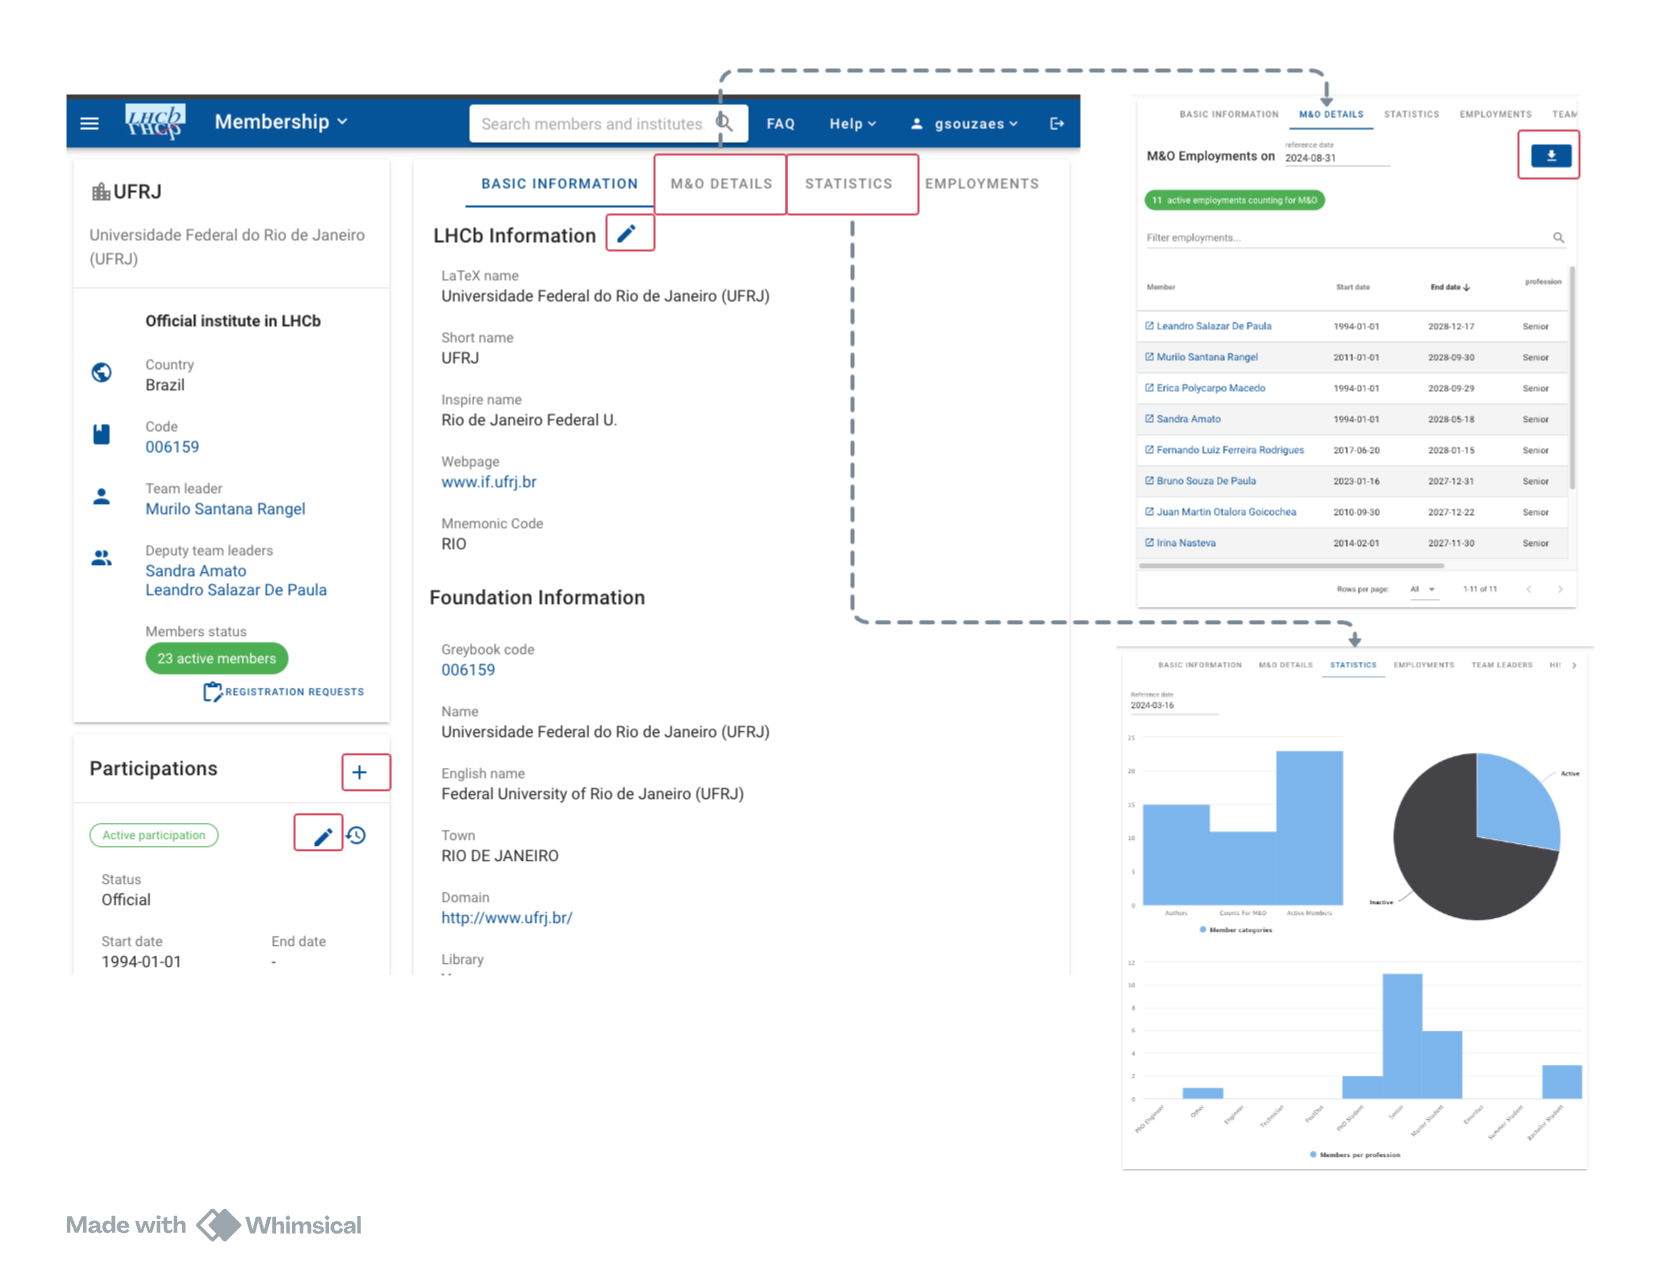
\includegraphics[width=1\linewidth]{figuras/mb_institute_profile.png}
    \caption{UFRJ Institute profile.}
    \label{fig:mb_institute_profile}
\end{figure}

\paragraph{} While Figure \ref{fig:wf_management_page} introduces the interfaces for workflow management, additional interfaces facilitate the management of all available workflows. Specifically, the management page for the Change Profession Workflow is shown in Figure \ref{fig:change_profession_wf}. Through this interface, Team Leaders and the Secretariat can review the list of all active processes. Analogous interfaces are available for managing the Change Institute Workflow, as well as the New Employment and Extend Employment Workflows, streamlining the oversight and administration of these processes.

\begin{figure} [H]
    \centering
    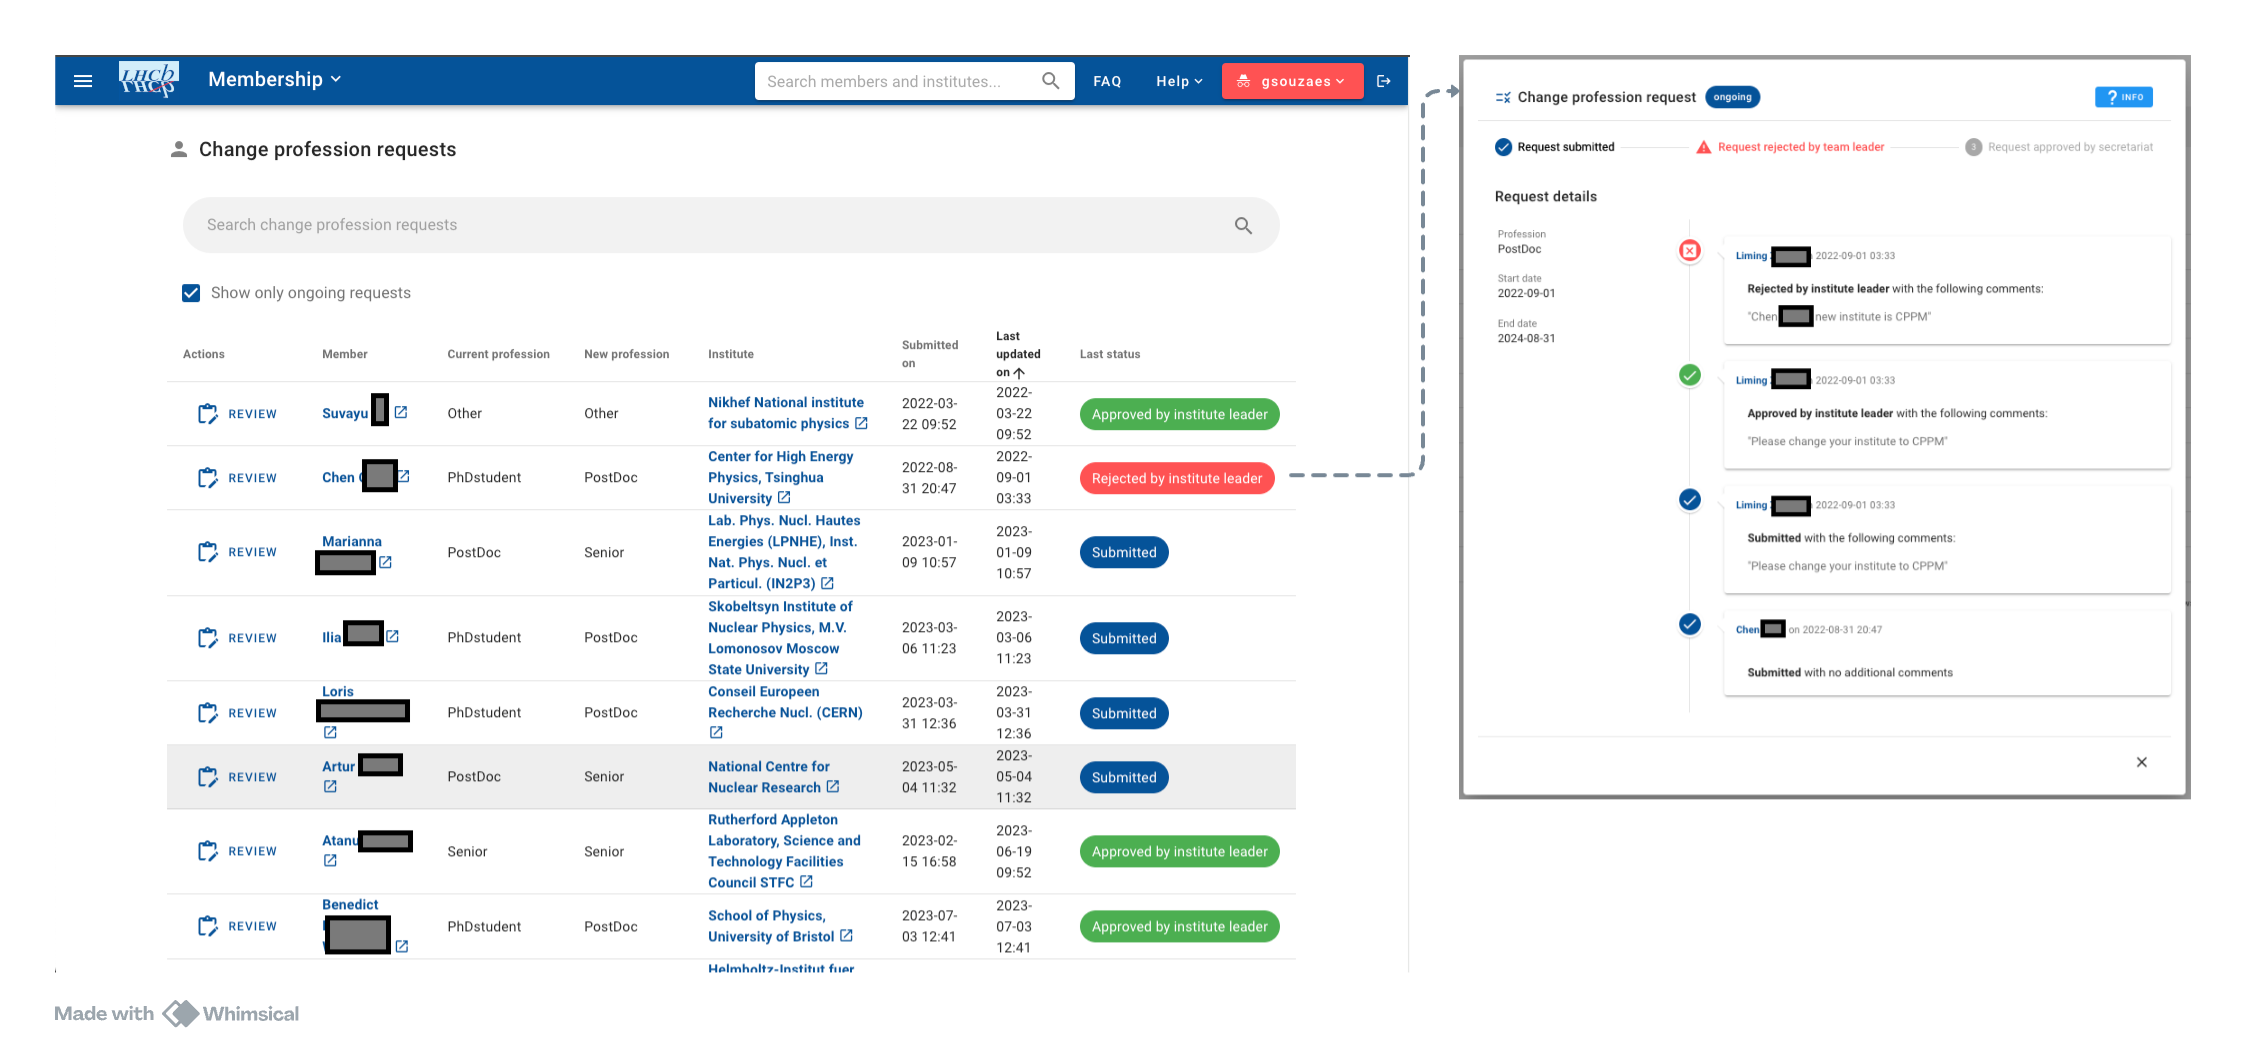
\includegraphics[width=1\linewidth]{figuras/change_profession_wf.png}
    \caption{Change Profession Request being reviewed.}
    \label{fig:change_profession_wf}
\end{figure}

\paragraph{} Graphs were introduced in the Vue-based version of the Membership system, as illustrated in Figure \ref{fig:mb_institute_profile}. These visualizations are also featured on public pages, for example, the Collaboration Map, which displays the number of LHCb participants, as depicted in Figure \ref{fig:collaboration_map}. Additionally, the Glance team collaborated with the ECGD (LHCb's Early Career, Gender \& Diversity Office) to generate graphs that analyze the gender distribution within LHCb, shown in Figure \ref{fig:gender}.

\begin{figure} [H]
    \centering
    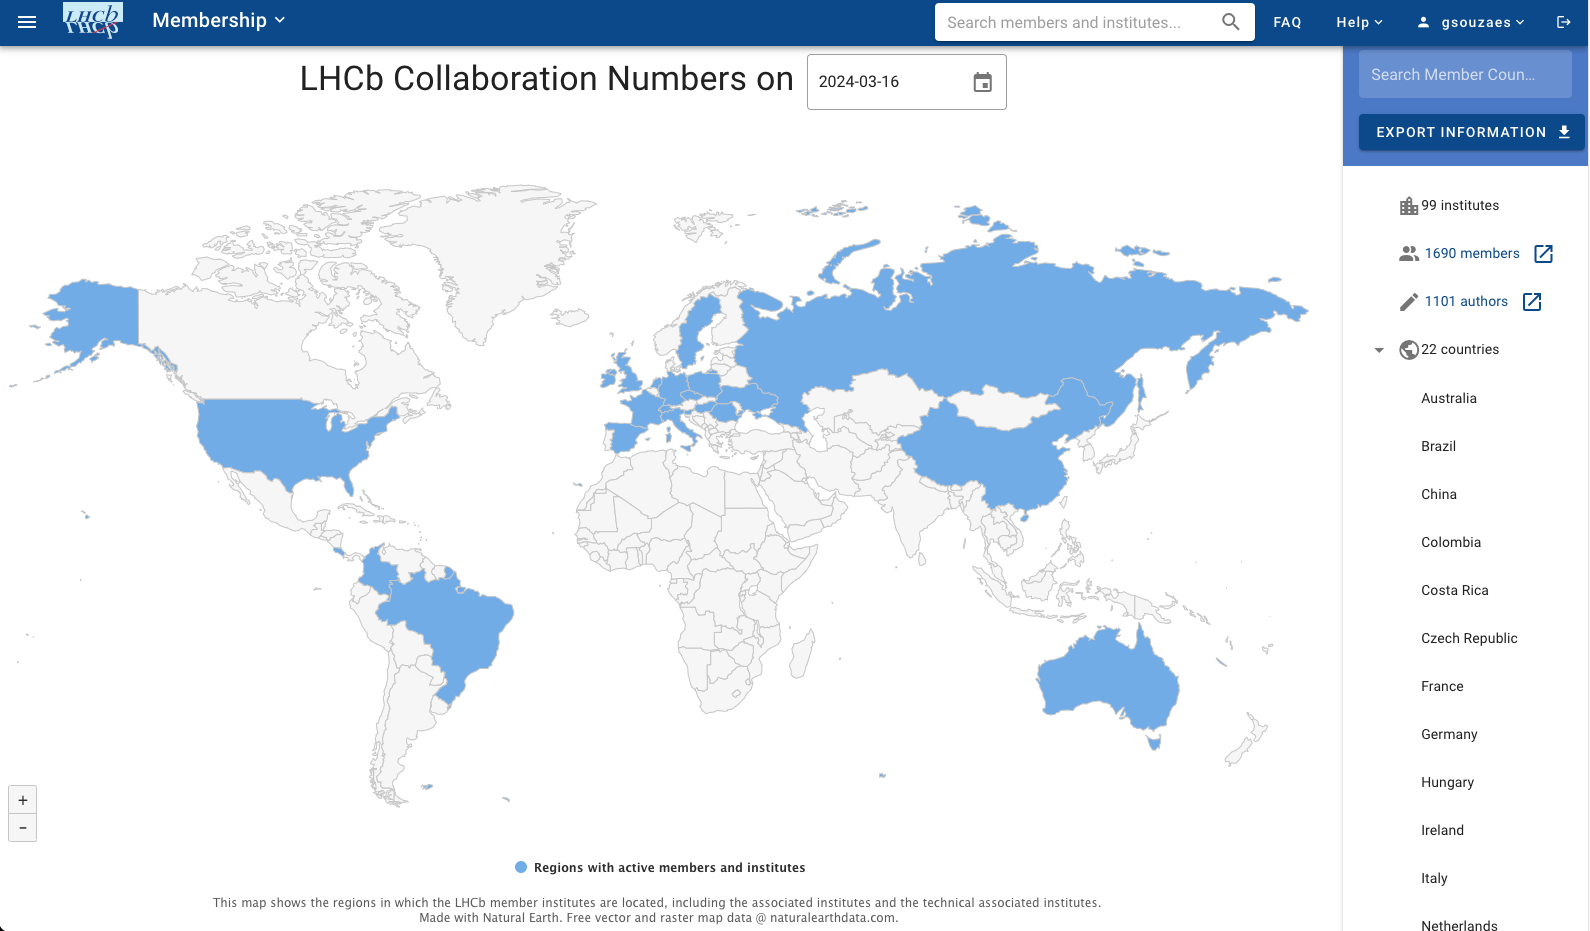
\includegraphics[width=1\linewidth]{figuras/collaboration_map.png}
    \caption{Countries that participate in the LHCb experiment.}
    \label{fig:collaboration_map}
\end{figure}


\begin{figure} [H]
    \centering
    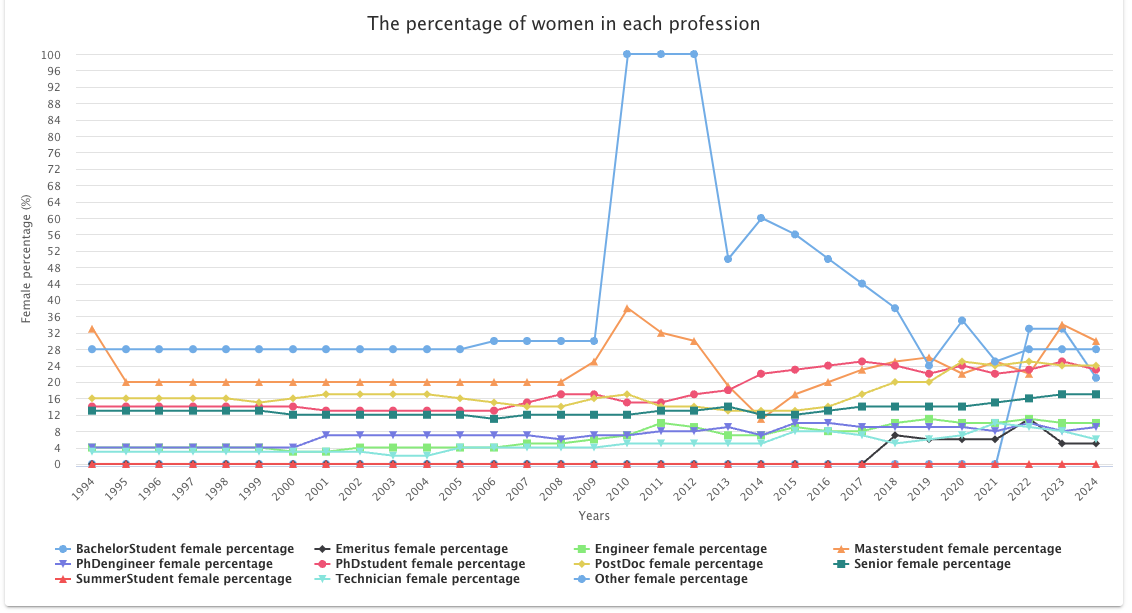
\includegraphics[width=1\linewidth]{figuras/gender.png}
    \caption{\textbf{Not real} (mocked) gender distribution data presented in the Membership.}
    \label{fig:gender}
\end{figure}

\paragraph{} Search interfaces for Appointments, Members, Institutes, and Employments facilitate data retrieval for the system's primary entities. Figure \ref{fig:homepage} illustrates the system's Homepage, which indexes all available views. From this central hub, users can navigate to specific search interfaces and access their Member and Institute profiles.

\begin{figure} [H]
    \centering
    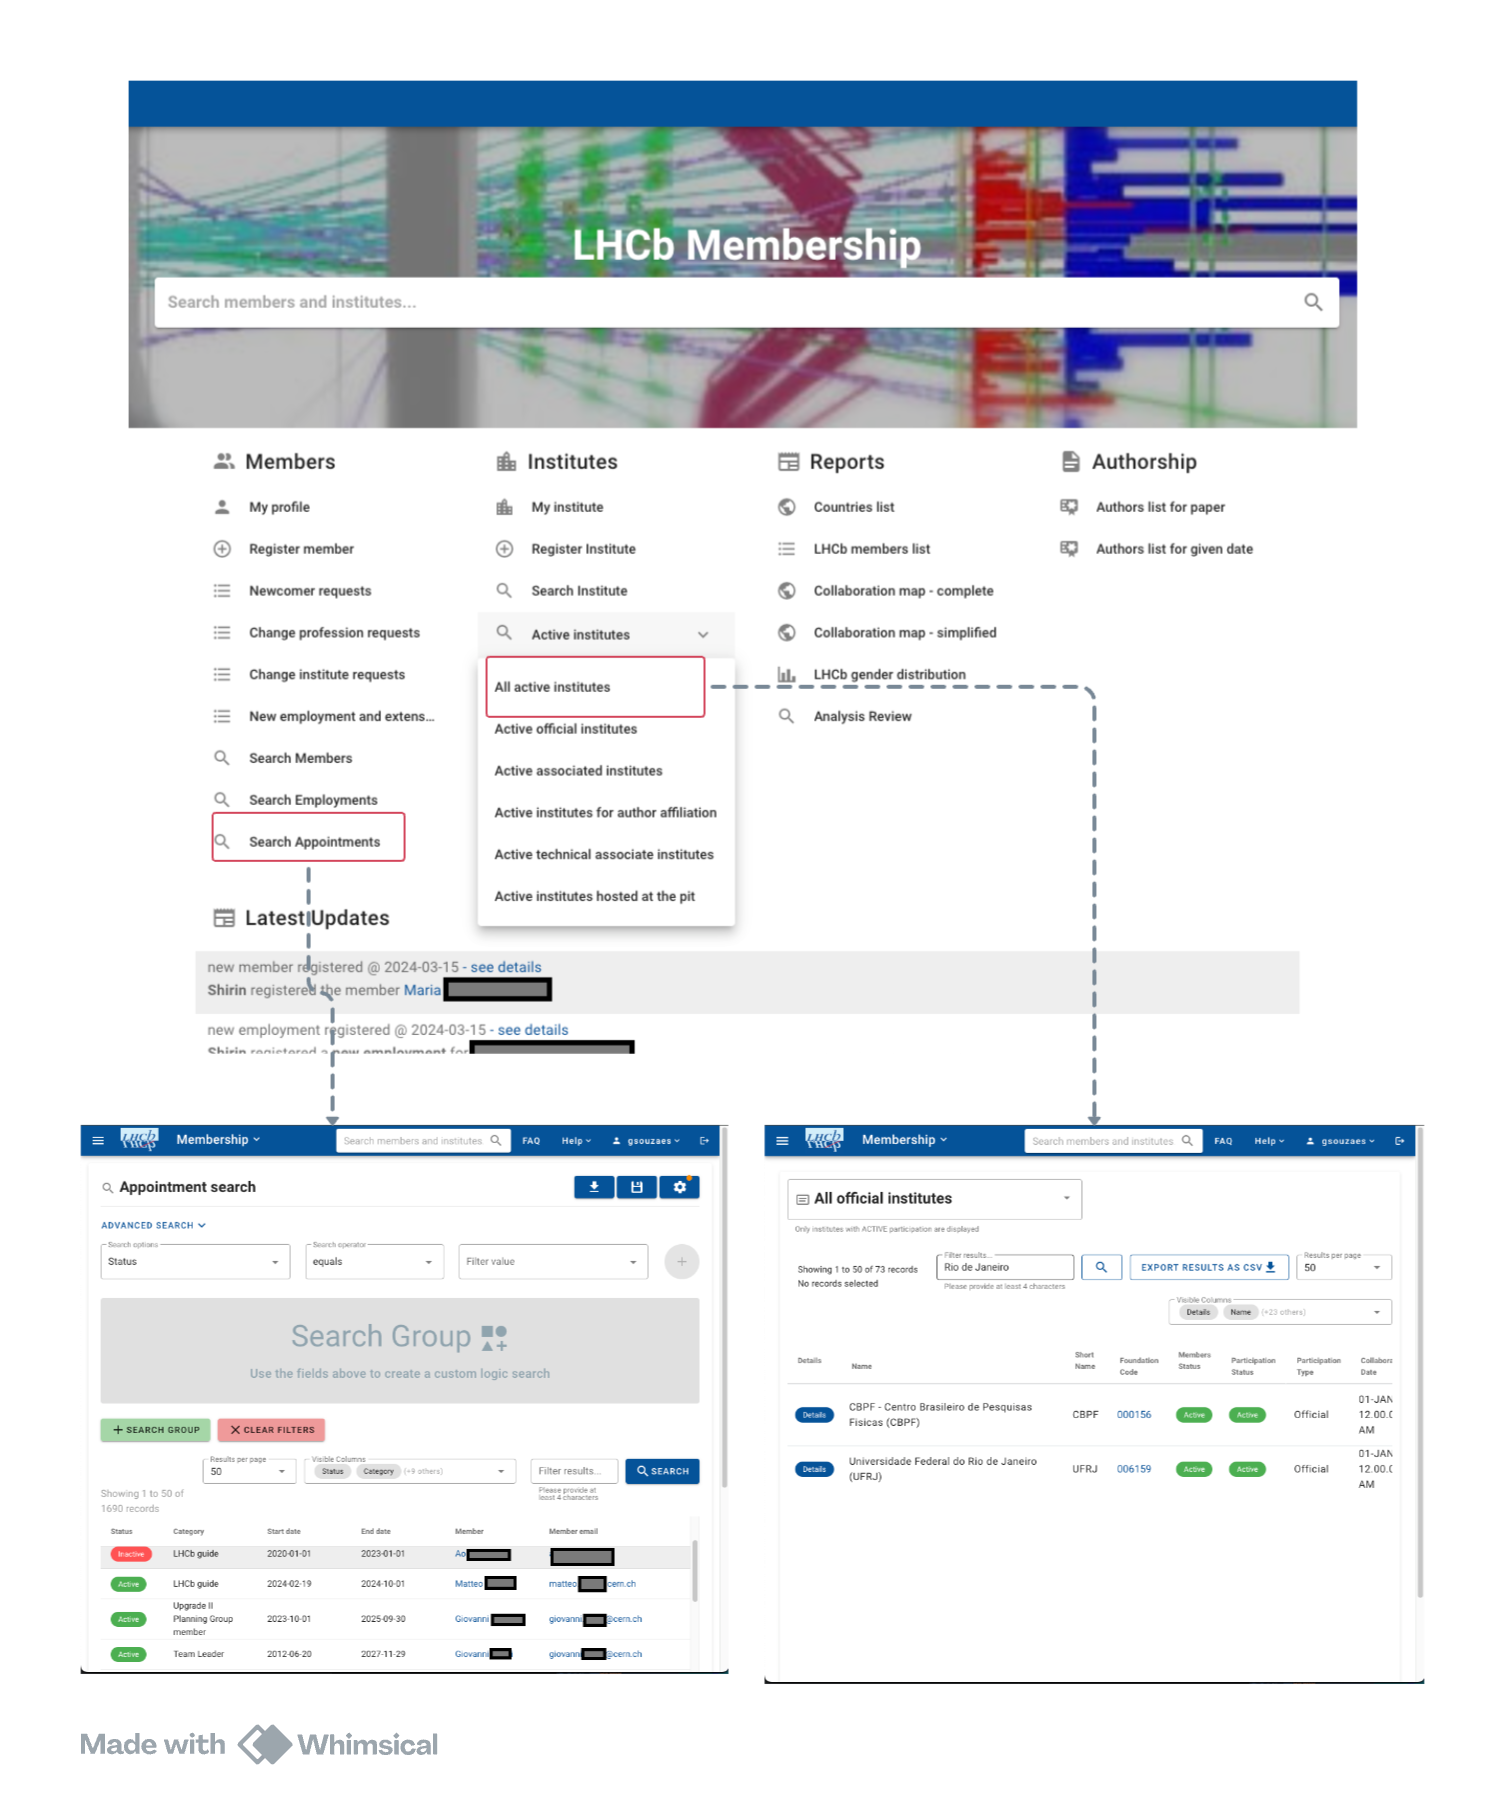
\includegraphics[width=1\linewidth]{figuras/homepage.png}
    \caption{LHCb Membership homepage and search interfaces.}
    \label{fig:homepage}
\end{figure}


\paragraph{} Data reports, including reminders for necessary actions, are dispatched via email through code in the Infrastructure Layer. This layer utilizes the same Application Layer Repository interfaces that the web Controller employs to display information in HTTP response bodies. A frequently dispatched email report highlights potential discrepancies between the Membership database and CERN's HR database, as depicted in Figure \ref{fig:email_report}. This inconsistencies report is sent to the Secretariat every Monday, enabling them to address and resolve them.

\begin{figure} [H]
    \centering
    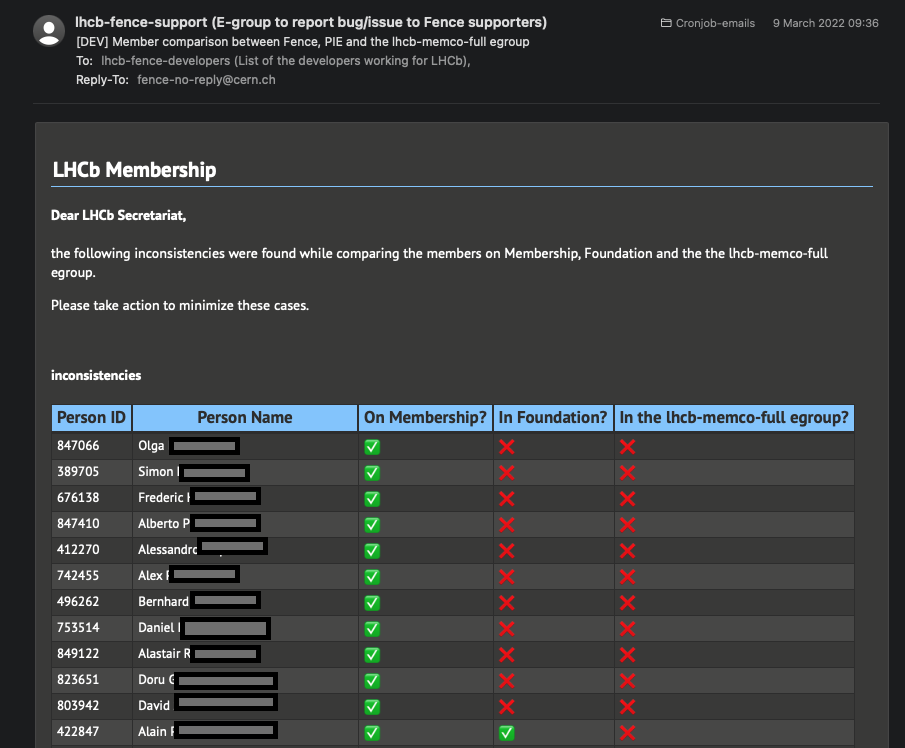
\includegraphics[width=0.8\linewidth]{figuras/email_report.png}
    \caption{Membership inconsistencies report sent weekly via email.}
    \label{fig:email_report}
\end{figure}